\documentclass[12pt]{article}

\usepackage{hcmus-report-template}

% Disable indentation on new paragraphs
\setlength{\parindent}{0pt}

% Line spacing 1.5
\renewcommand{\baselinestretch}{1.5}

% Graphic path — trỏ vào thư mục img/
\graphicspath{{img/}}

% To use Times font family, uncomment this row
% \usepackage{mathptmainmx}

% To use roman section / subsection, uncomment these rows
%\renewcommand{\thesection}{\Roman{section}}
%\renewcommand{\thesubsection}{\thesection.\Roman{subsection}}

% Define course name, report name and report title.
\newcommand{\coursename}{Nhập môn Dữ liệu lớn}
\newcommand{\reportname}{Lab 01: Hadoop Cluster \& WordCount}
\newcommand{\reporttitle}{BÁO CÁO ĐỒ ÁN}

\newcommand{\studentname}{23120099 - Lê Xuân Trí}
\newcommand{\teachername}{Thầy Trần Huy Bân}

% Header
\lhead{\reporttitle}
\rhead{
Trường Đại học Khoa học Tự nhiên - ĐHQG HCM\\
\coursename
}

% Footer
%\newcommand{\leftfooter}{\LaTeX\ by \href{https://github.com/trhgquan}{Quan, Tran Hoang}}
%\lfoot{\leftfooter}

% ============ DOCUMENT ============

% --- Extra packages from report.tex ---
\usepackage{float}
\usepackage{booktabs}
\usepackage{tabularx}
\usepackage{longtable}
\usepackage{xcolor}
\definecolor{codebg}{RGB}{245,245,245}
\usepackage{minted}
\usemintedstyle{friendly}
\setminted{
  bgcolor=codebg,
  fontsize=\footnotesize,
  breaklines=true,
  frame=single,
  framesep=2mm,
}
\usepackage{enumitem}
\usepackage{titlesec}
\usepackage{caption}
\usepackage{needspace}

\begin{document}

\pagenumbering{roman}

% ============================================================
% TRANG BÌA (inline từ content/title.tex)
% ============================================================
\begin{titlepage}
\newcommand{\HRule}{\rule{\linewidth}{0.5mm}}
\centering

\textsc{\LARGE đại học quốc gia tphcm}\\[0.5cm]
\textsc{\Large trường đại học khoa học tự nhiên}\\[0.5cm]
\textsc{\large khoa công nghệ thông tin}\\[0.4cm]


\includegraphics[scale=.40]{hcmus-logo.png}\\[0.1cm] 

\HRule \\[0.3cm]
{ 
\huge{\bfseries{\reporttitle}}\\[0.5cm]
\large{\bfseries{Chủ đề: \reportname}}
}\\[0.4cm]
\HRule \\[0.5cm]



\textbf{\large Môn học: \coursename}\\[0.5cm]

\begin{minipage}[t]{0.4\textwidth}
\begin{flushleft} \large
\emph{Sinh viên thực hiện:}\\
\studentname
\end{flushleft}
\end{minipage}
~
\begin{minipage}[t]{0.4\textwidth}
\begin{flushright} \large
\emph{Giảng viên hướng dẫn:} \\
\teachername
\end{flushright}
\end{minipage}\\[1cm]

{\large \today}\\[1cm]



\vfill
\end{titlepage}

\tableofcontents
\pagebreak
% \listoftables
\pagebreak
\listoffigures
\pagebreak

\pagenumbering{arabic}
\setcounter{page}{1}

% ============================================================
% PHẦN 1: CÀI ĐẶT HADOOP PSEUDO-DISTRIBUTED
% ============================================================
\section{Cài đặt Hadoop Pseudo-Distributed}

Phần này trình bày toàn bộ quá trình tôi cài đặt và cấu hình Hadoop 3.4.0 ở chế độ
pseudo-distributed trên máy cá nhân chạy Arch Linux. Mỗi bước đều được ghi lại kèm
lệnh thực thi và ảnh chụp màn hình minh hoạ.

% ------------------------------------------------------------
\subsection{Môi trường hệ thống}

Tôi sử dụng Arch Linux — một bản phân phối rolling-release cho phép luôn cập nhật các
gói phần mềm lên phiên bản mới nhất mà không cần cài đặt lại toàn bộ hệ thống. Nhân
Linux đang dùng là phiên bản mới nhất từ kho chính thức của Arch, đảm bảo hỗ trợ đầy
đủ các tính năng phần cứng hiện đại. Arch Linux được chọn vì tính minh bạch, tài liệu
ArchWiki phong phú, và khả năng kiểm soát hoàn toàn các gói cài đặt thông qua trình
quản lý gói \texttt{pacman}.

Để kiểm tra thông tin nhân và kiến trúc hệ thống, tôi chạy lệnh:

\begin{minted}{bash}
uname -a
\end{minted}

\begin{figure}[H]
  \centering
  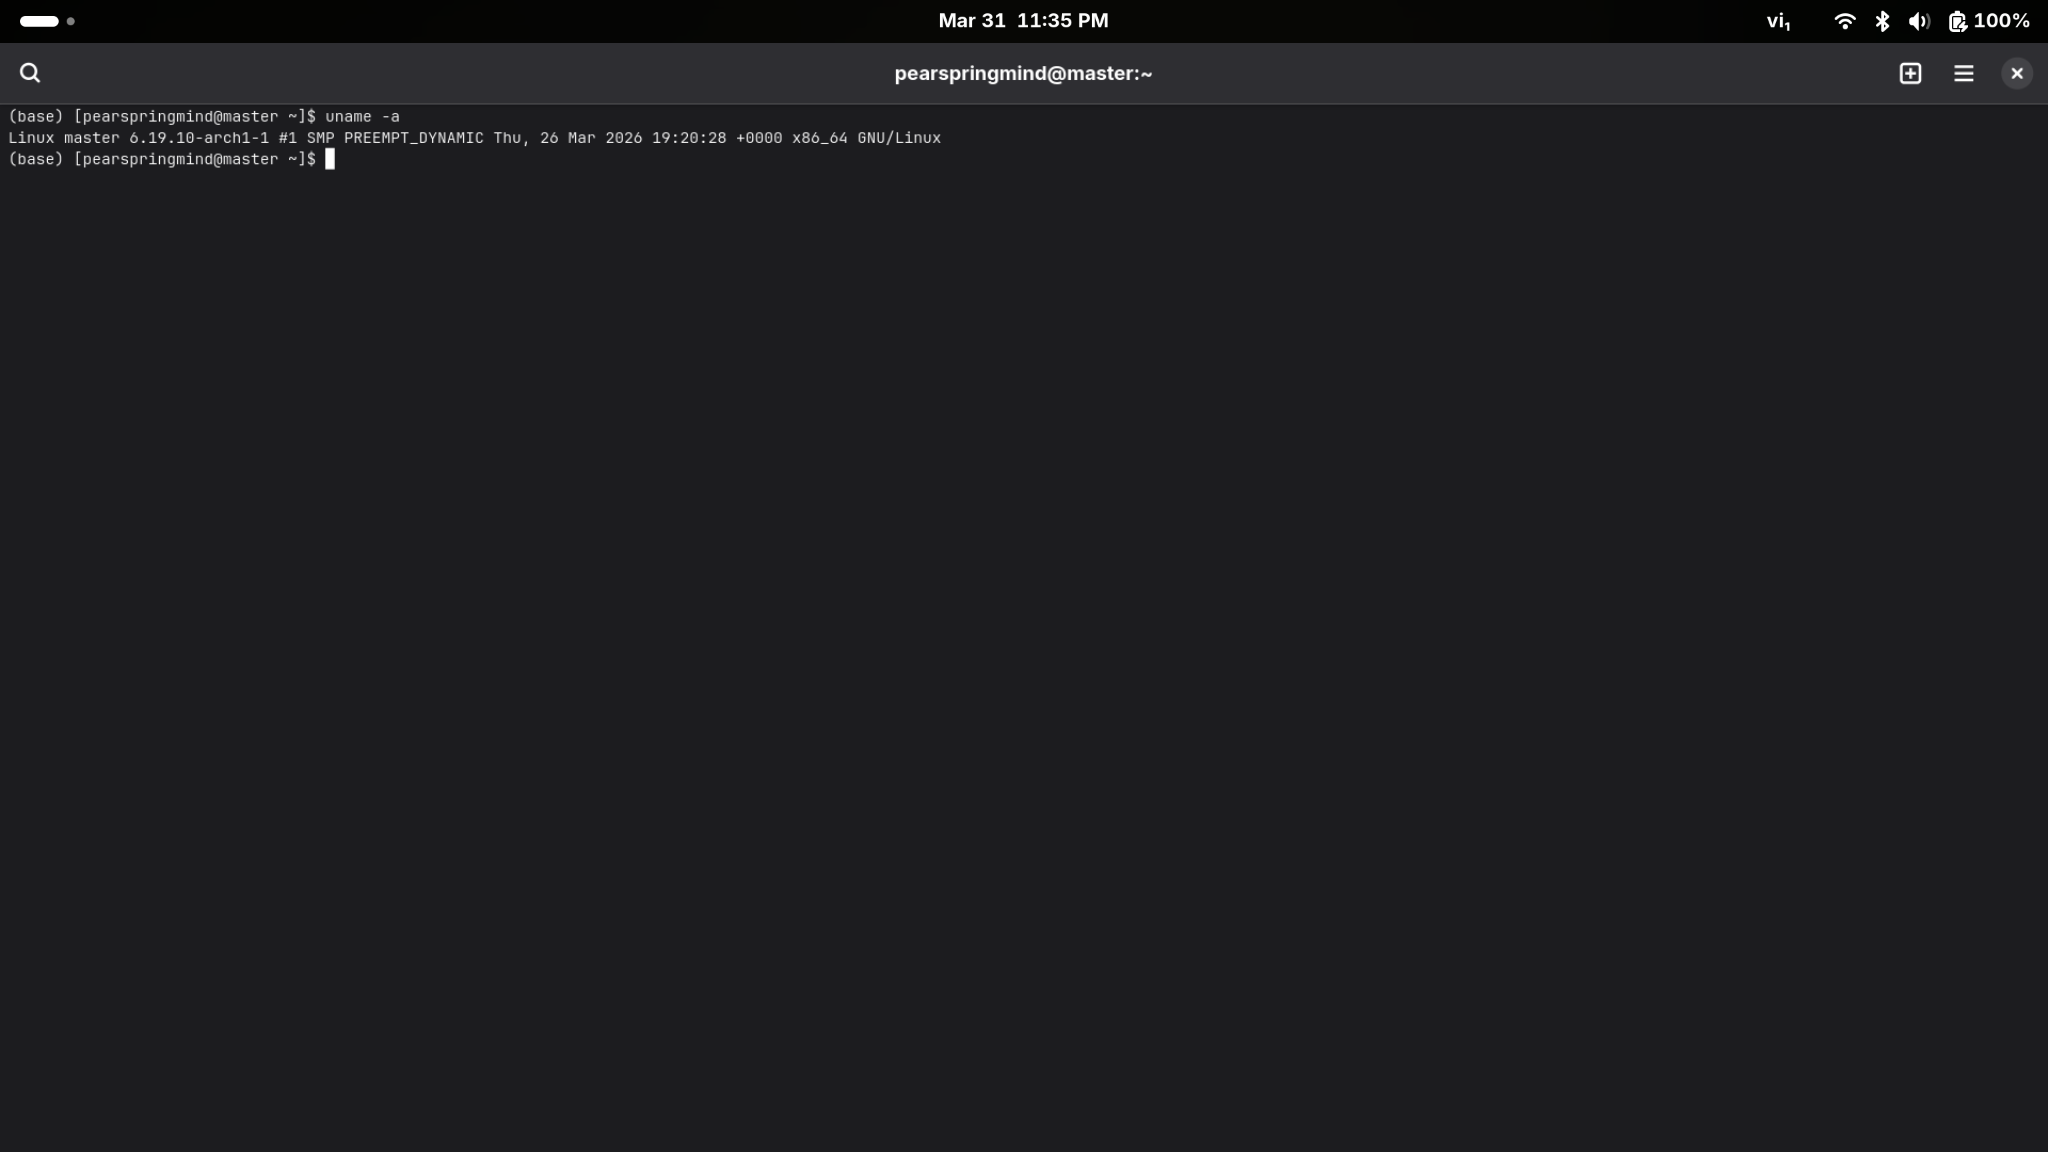
\includegraphics[width=\textwidth]{uname.png}
  \caption{Kết quả kiểm tra nhân và kiến trúc hệ thống bằng lệnh uname -a}
  \label{fig:uname}
\end{figure}

Đồng thời, để hệ thống các node trong cụm có thể giao tiếp với nhau ổn định, tôi kiểm tra địa chỉ IP hiện tại trên giao diện mạng bằng lệnh \texttt{ip addr}:

\begin{minted}{bash}
ip addr
\end{minted}

\begin{figure}[H]
  \centering
  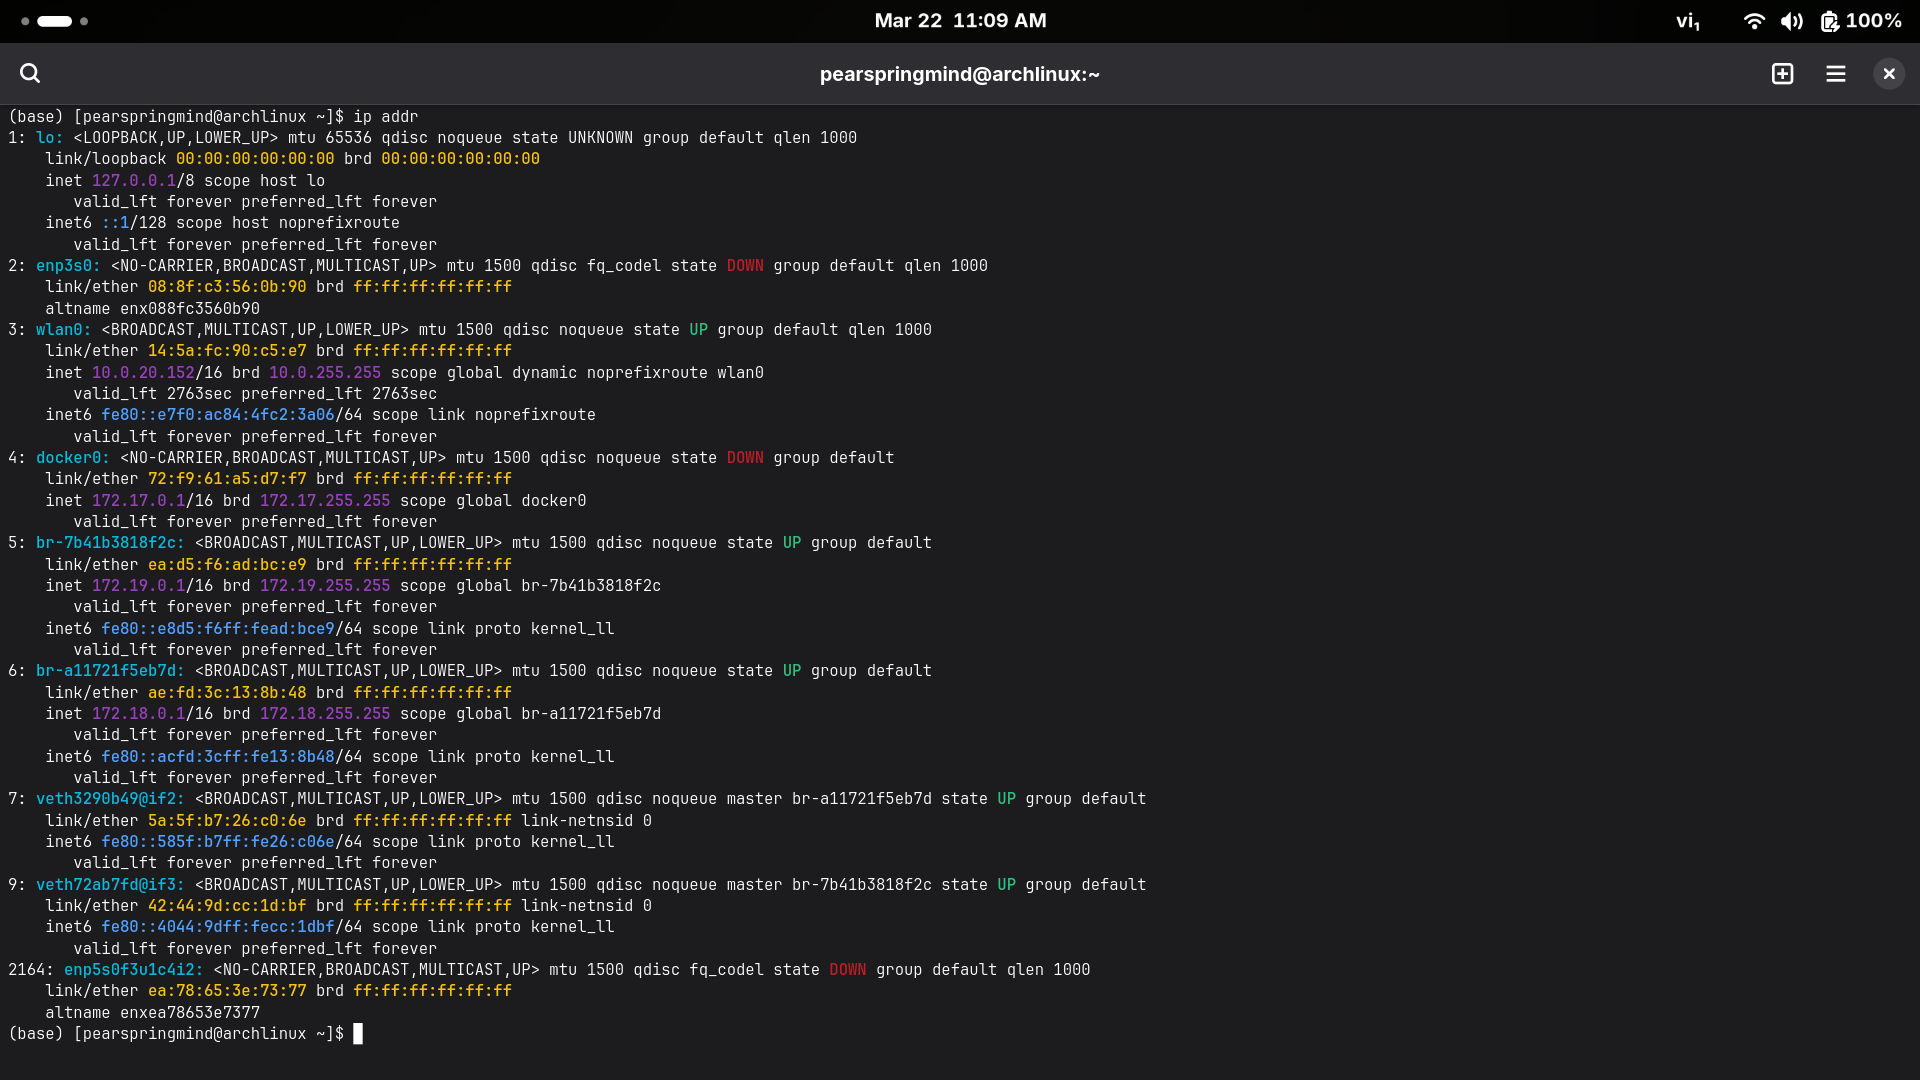
\includegraphics[width=\textwidth]{08-ip-proof.png}
  \caption{Xác minh địa chỉ IP của hệ thống phục vụ cấu hình Hadoop}
  \label{fig:ip-addr}
\end{figure}

% ------------------------------------------------------------
\subsection{Cài đặt Java và Scala}

Hadoop yêu cầu Java Runtime Environment để vận hành vì toàn bộ hệ sinh thái Hadoop
được viết bằng Java. Tôi chọn OpenJDK 11 vì đây là phiên bản LTS được Hadoop 3.4.0
hỗ trợ chính thức và đã được kiểm chứng ổn định. Scala được cài đặt để phục vụ cho
việc lập trình WordCount bằng Apache Spark ở phần sau, vì Spark được viết bằng Scala
và hỗ trợ API Scala tốt nhất.

\begin{minted}{bash}
sudo pacman -S jre11-openjdk jdk11-openjdk
yay -S scala
java -version
scala -version
\end{minted}

\begin{figure}[H]
  \centering
  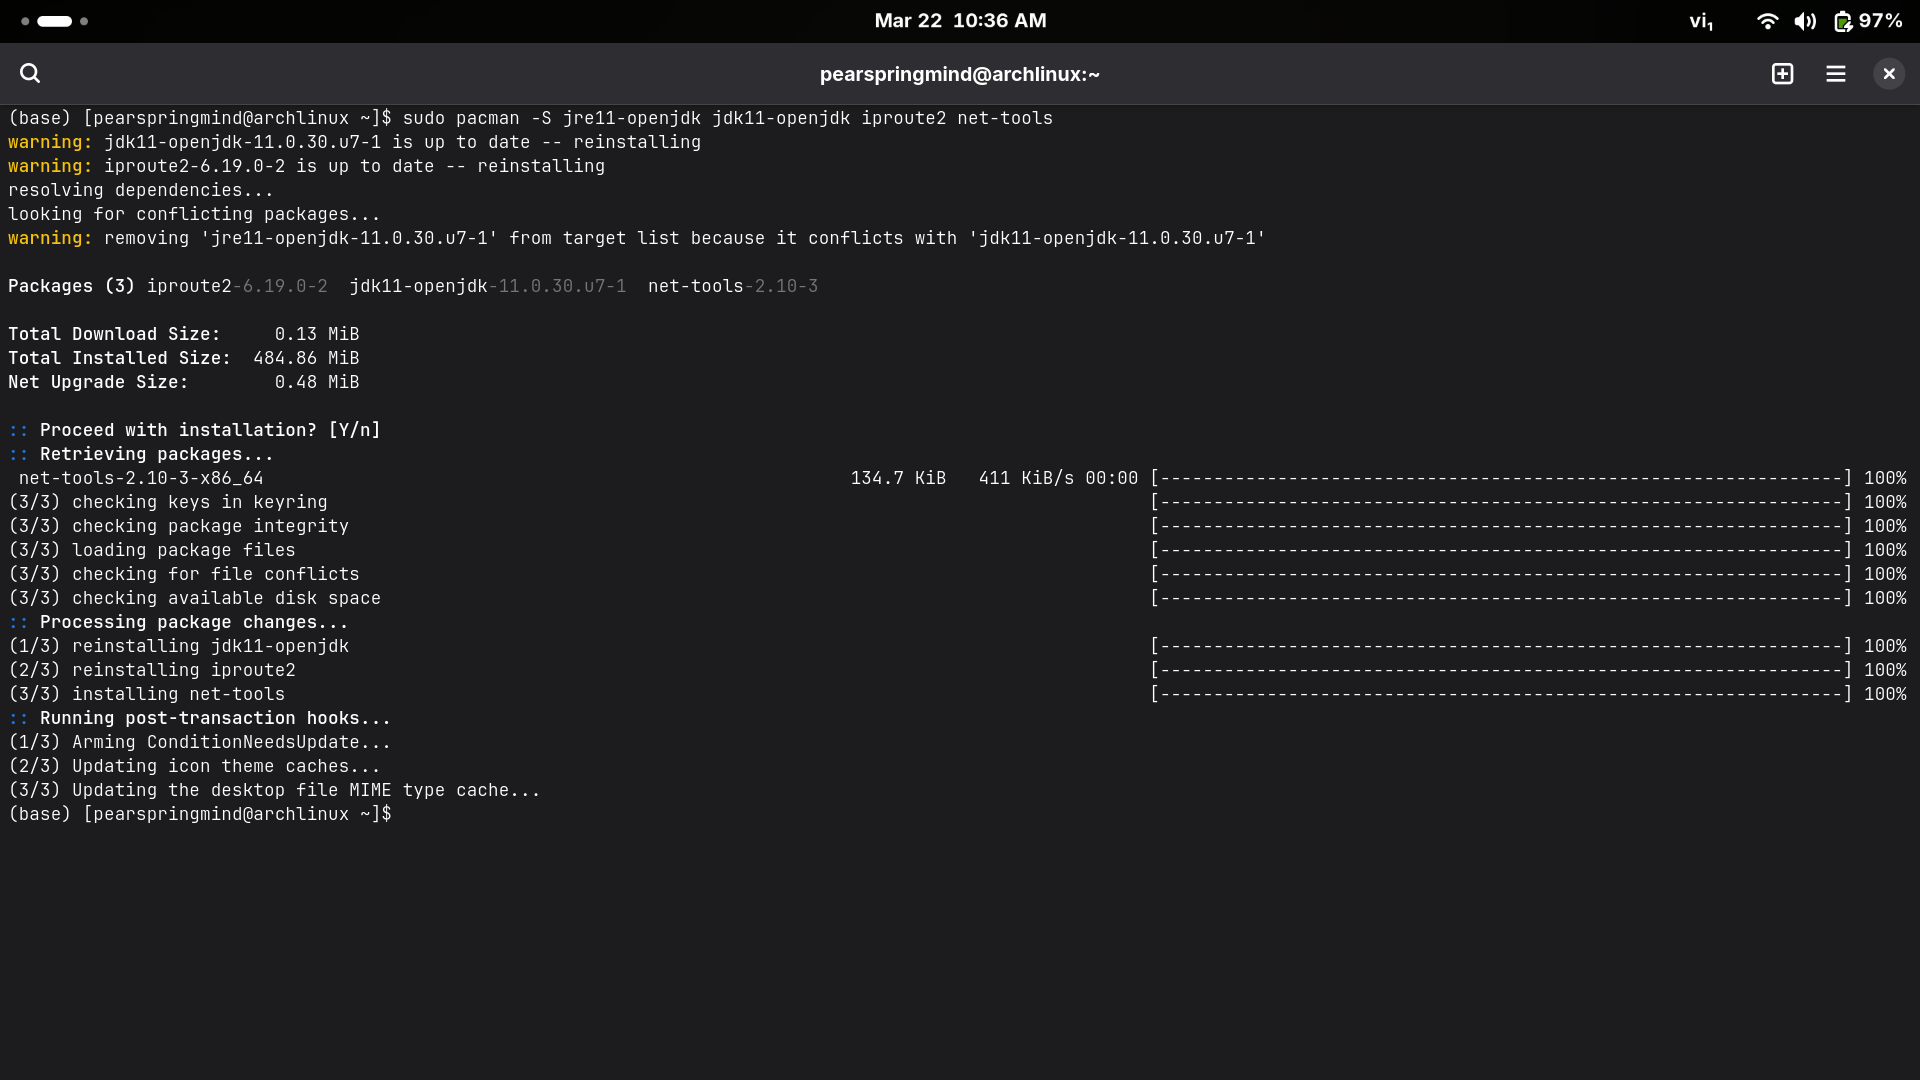
\includegraphics[width=0.48\textwidth]{01-java-install.png}
  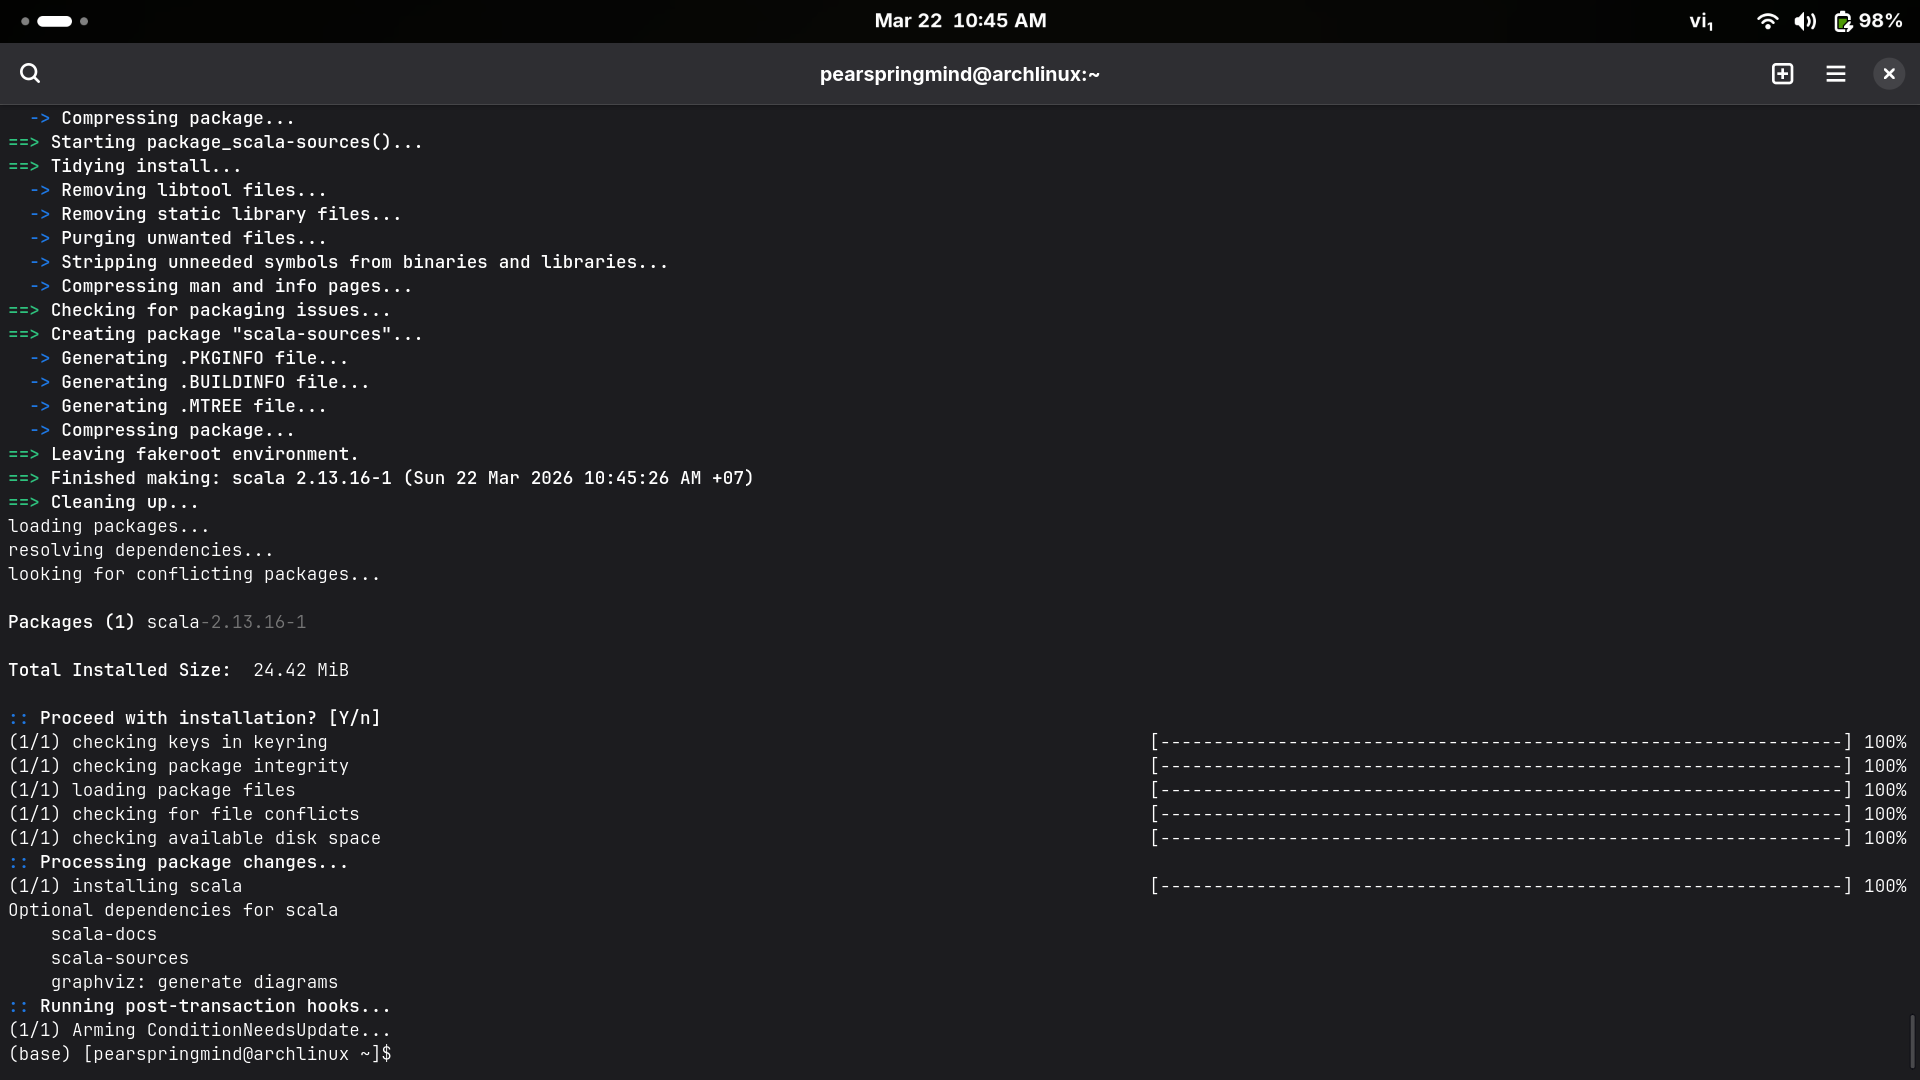
\includegraphics[width=0.48\textwidth]{02-scala-install.png}
  \caption{Cài đặt Java SE 11 và Scala thành công}
  \label{fig:java-scala}
\end{figure}

% ------------------------------------------------------------
\subsection{Tải và giải nén Hadoop}

Tôi tải Hadoop phiên bản 3.4.0 — phiên bản ổn định mới nhất tại thời điểm thực hiện
bài lab — trực tiếp từ máy chủ phân phối chính thức của Apache. Sau khi tải về, file
nén \texttt{.tar.gz} được giải nén vào thư mục \texttt{/opt/} theo quy ước đặt phần
mềm bên thứ ba trên hệ thống Linux. Cuối cùng, tôi thay đổi quyền sở hữu thư mục
Hadoop để tài khoản người dùng hiện tại có toàn quyền đọc, ghi và thực thi.

\begin{minted}{bash}
wget https://downloads.apache.org/hadoop/common/hadoop-3.4.0/hadoop-3.4.0.tar.gz
sudo tar -xzvf hadoop-3.4.0.tar.gz -C /opt/
sudo chown -R $USER:$USER /opt/hadoop
\end{minted}

\begin{figure}[H]
  \centering
  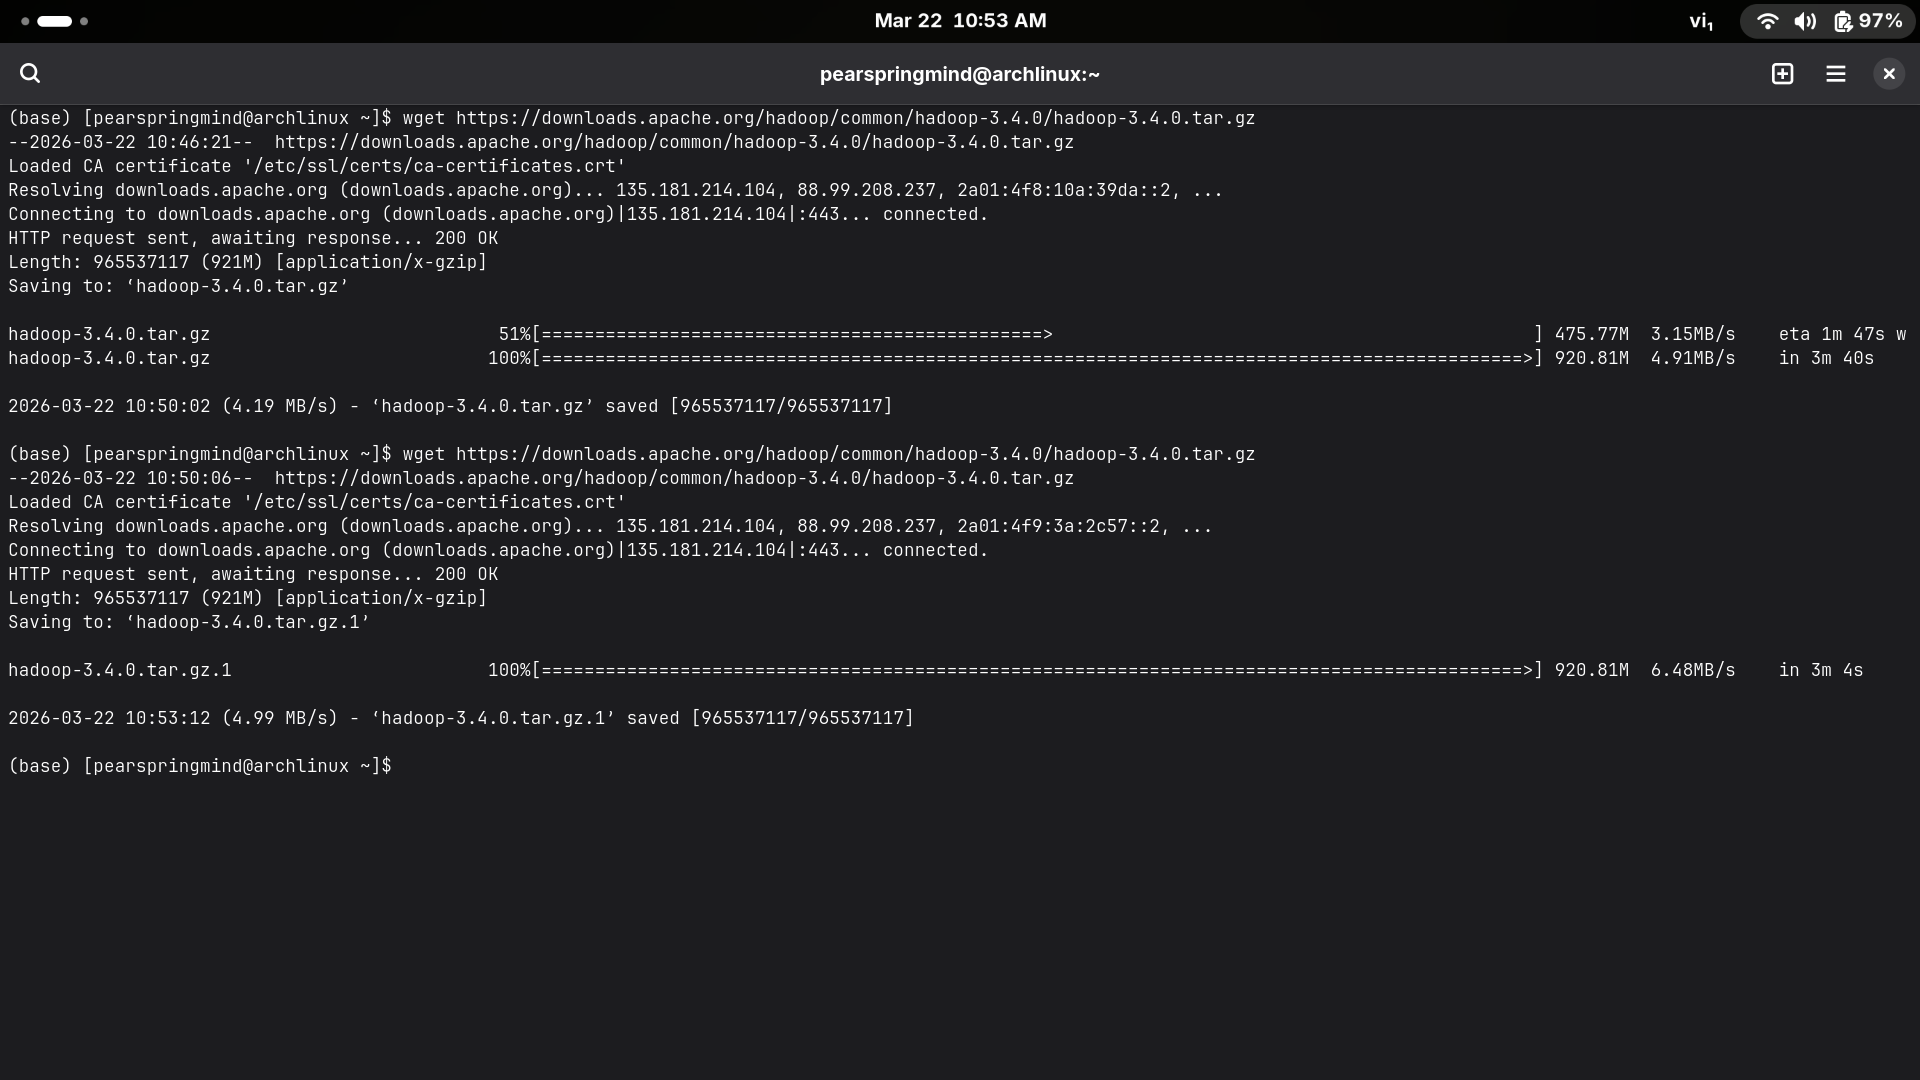
\includegraphics[width=0.48\textwidth]{03-hadoop-download.png}
  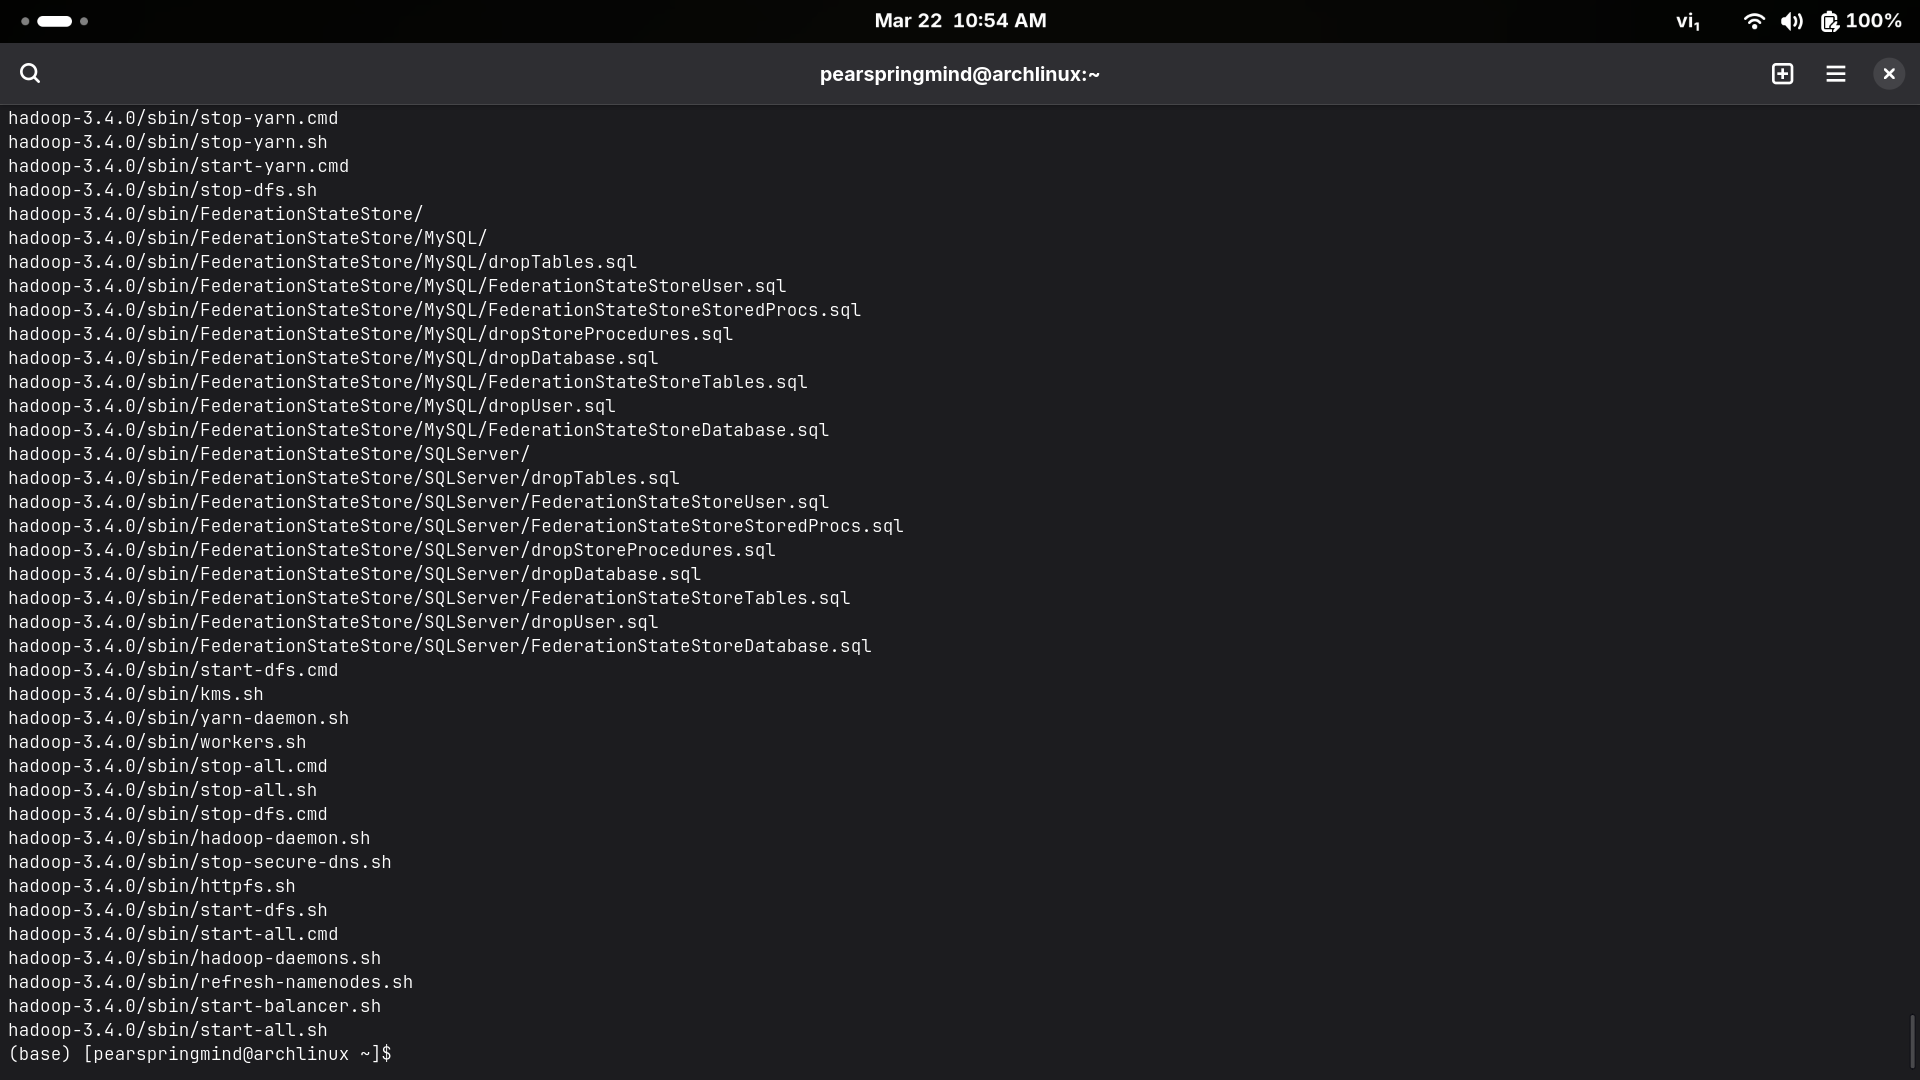
\includegraphics[width=0.48\textwidth]{04-hadoop-list.png}
  \caption{Tải và kiểm tra bộ cài Hadoop 3.4.0}
  \label{fig:hadoop-download}
\end{figure}

% ------------------------------------------------------------
\subsection{Cấu hình biến môi trường}

Các biến môi trường cần thiết để hệ thống và Hadoop tìm đúng đường dẫn đến Java và
các công cụ Hadoop. Biến \texttt{JAVA\_HOME} chỉ đường dẫn đến thư mục cài đặt JDK,
\texttt{HADOOP\_HOME} trỏ đến thư mục Hadoop đã giải nén, còn biến \texttt{PATH}
được bổ sung đường dẫn đến thư mục \texttt{bin} và \texttt{sbin} của Hadoop để có
thể gọi trực tiếp các lệnh như \texttt{hdfs}, \texttt{start-dfs.sh} từ bất kỳ đâu
trong terminal. Tôi thêm các dòng này vào cuối file \texttt{\textasciitilde/.bashrc}
để tự động nạp khi mở terminal mới.

\begin{minted}{bash}
export JAVA_HOME=/usr/lib/jvm/java-11-openjdk
export HADOOP_HOME=/opt/hadoop
export PATH=$PATH:$HADOOP_HOME/bin:$HADOOP_HOME/sbin
\end{minted}

\begin{figure}[H]
  \centering
  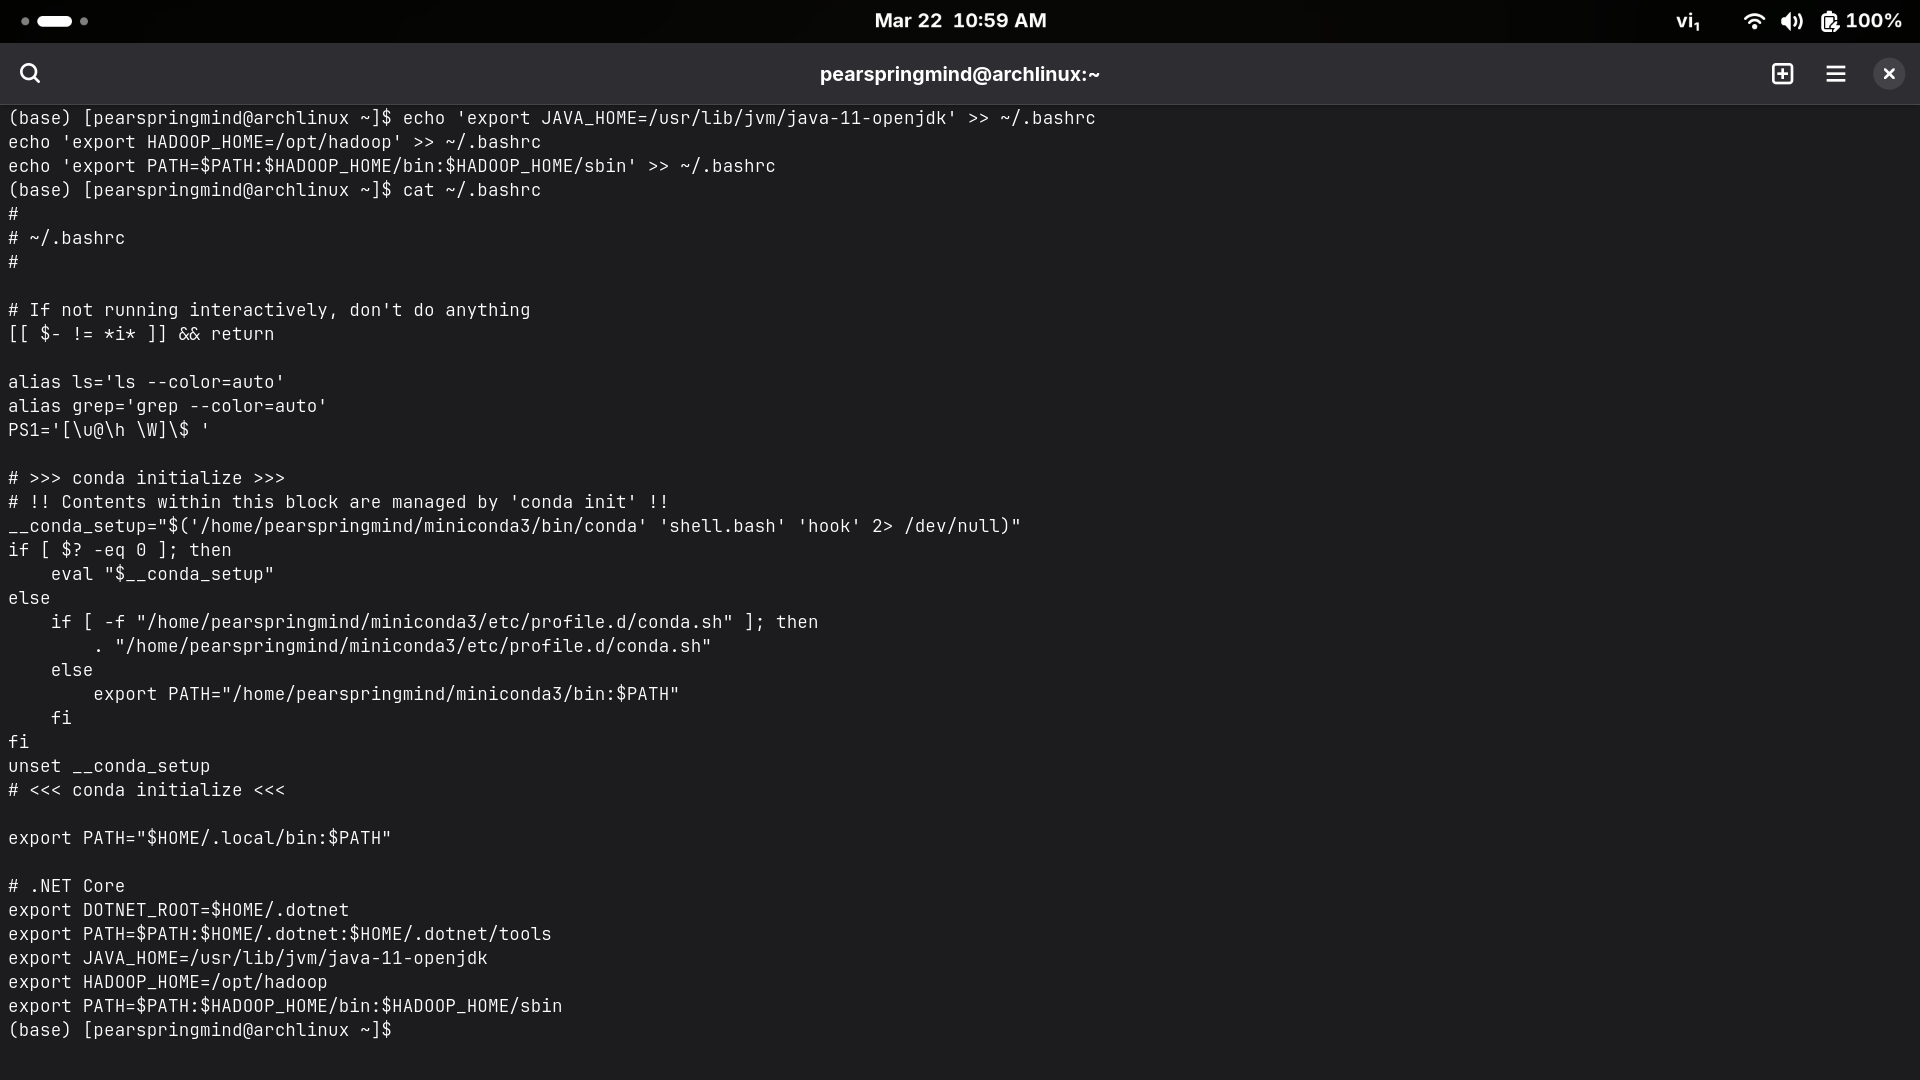
\includegraphics[width=0.48\textwidth]{05-env-vars.png}
  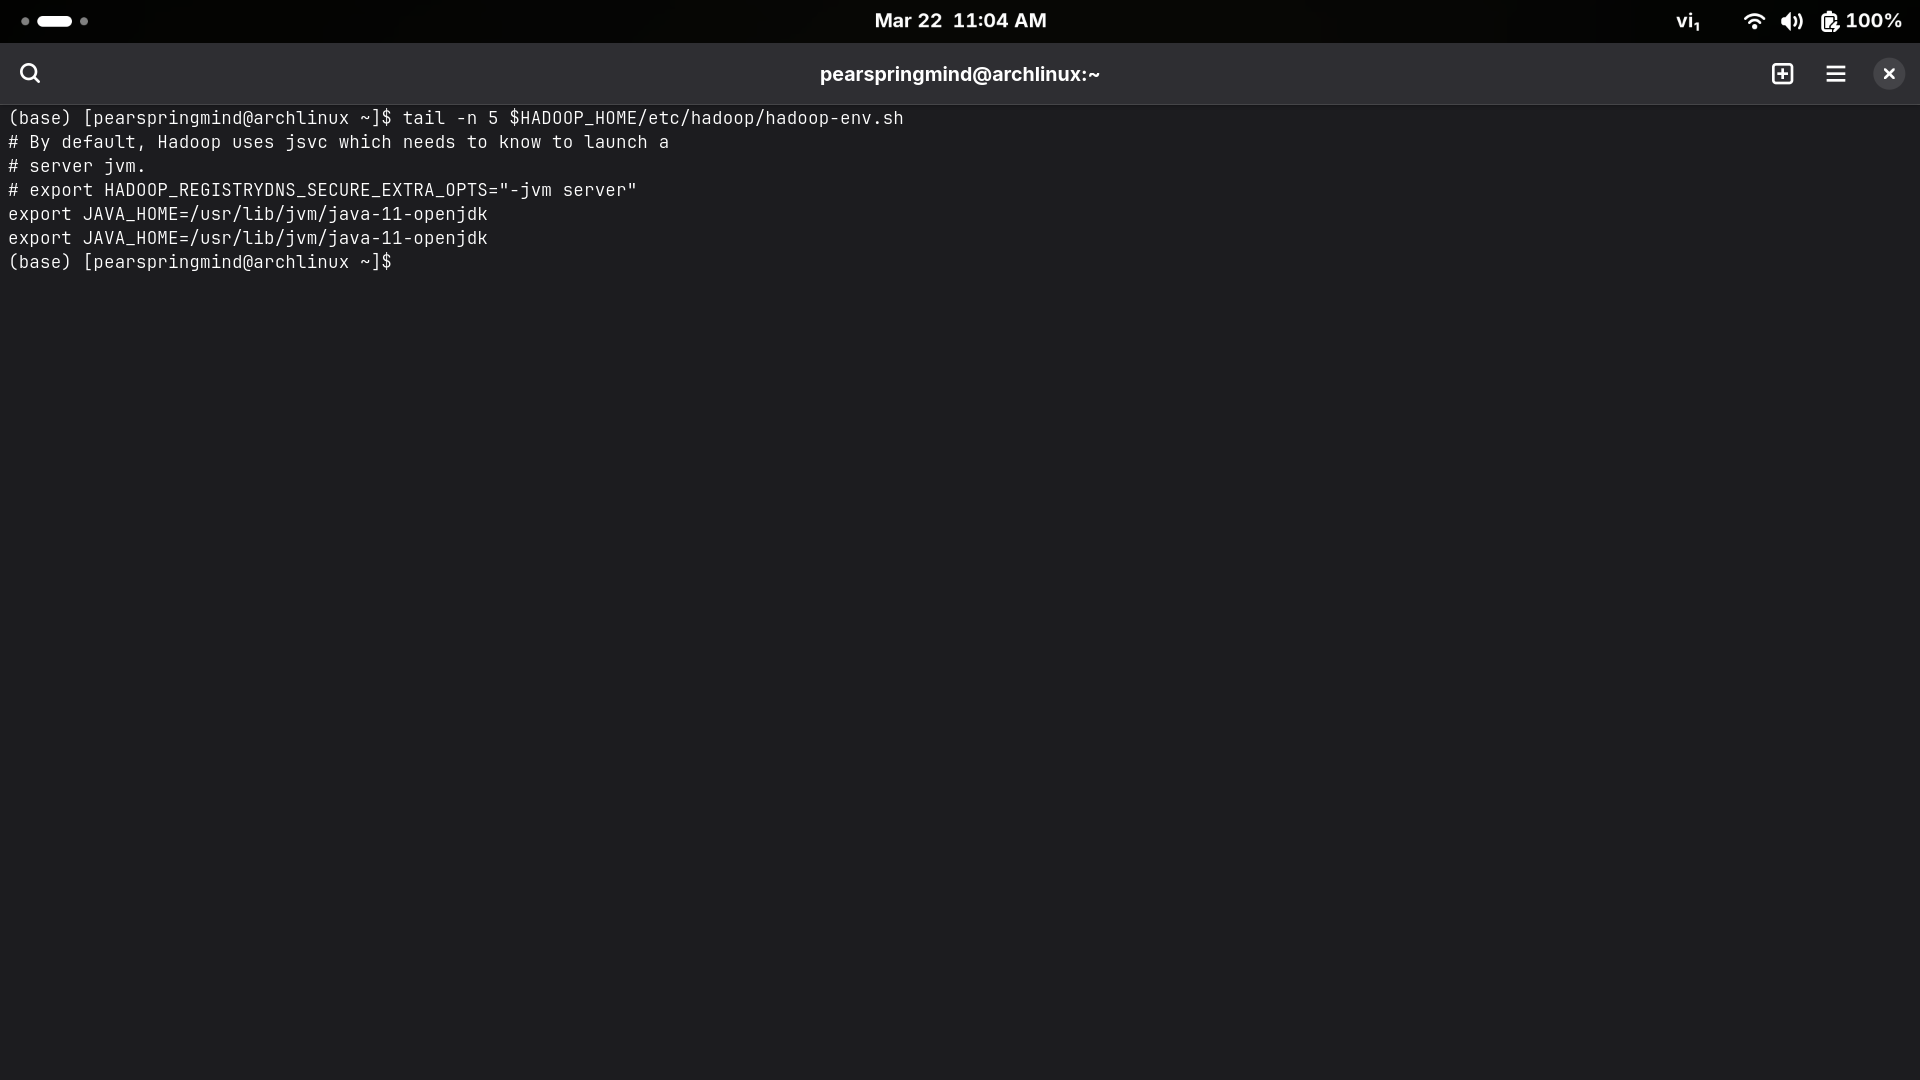
\includegraphics[width=0.48\textwidth]{06-hadoop-env-config.png}
  \caption{Cấu hình biến môi trường trong ~/.bashrc và hadoop-env.sh}
  \label{fig:env-vars}
\end{figure}

% ------------------------------------------------------------
\subsection{Cấu hình XML (core-site.xml, hdfs-site.xml)}

Hadoop sử dụng các file XML để cấu hình hành vi của từng thành phần. File
\texttt{core-site.xml} xác định địa chỉ mặc định của hệ thống file phân tán thông
qua thuộc tính \texttt{fs.defaultFS}; ở chế độ pseudo-distributed, tôi đặt giá trị
là \texttt{hdfs://localhost:9000}. File \texttt{hdfs-site.xml} cấu hình các thông số
của HDFS: \texttt{dfs.replication} được đặt bằng 1 vì chỉ có một node duy nhất,
\texttt{dfs.namenode.name.dir} chỉ đường dẫn lưu trữ metadata của NameNode, và
\texttt{dfs.datanode.data.dir} chỉ đường dẫn lưu trữ dữ liệu thực tế của DataNode.

\textbf{Nội dung file \texttt{core-site.xml}:}

\begin{minted}{xml}
<configuration>
  <property>
    <name>fs.defaultFS</name>
    <value>hdfs://localhost:9000</value>
  </property>
</configuration>
\end{minted}

\textbf{Nội dung file \texttt{hdfs-site.xml}:}

\begin{minted}{xml}
<configuration>
  <property>
    <name>dfs.replication</name>
    <value>1</value>
  </property>
  <property>
    <name>dfs.namenode.name.dir</name>
    <value>/opt/hadoop/data/namenode</value>
  </property>
  <property>
    <name>dfs.datanode.data.dir</name>
    <value>/opt/hadoop/data/datanode</value>
  </property>
</configuration>
\end{minted}

\begin{figure}[H]
  \centering
  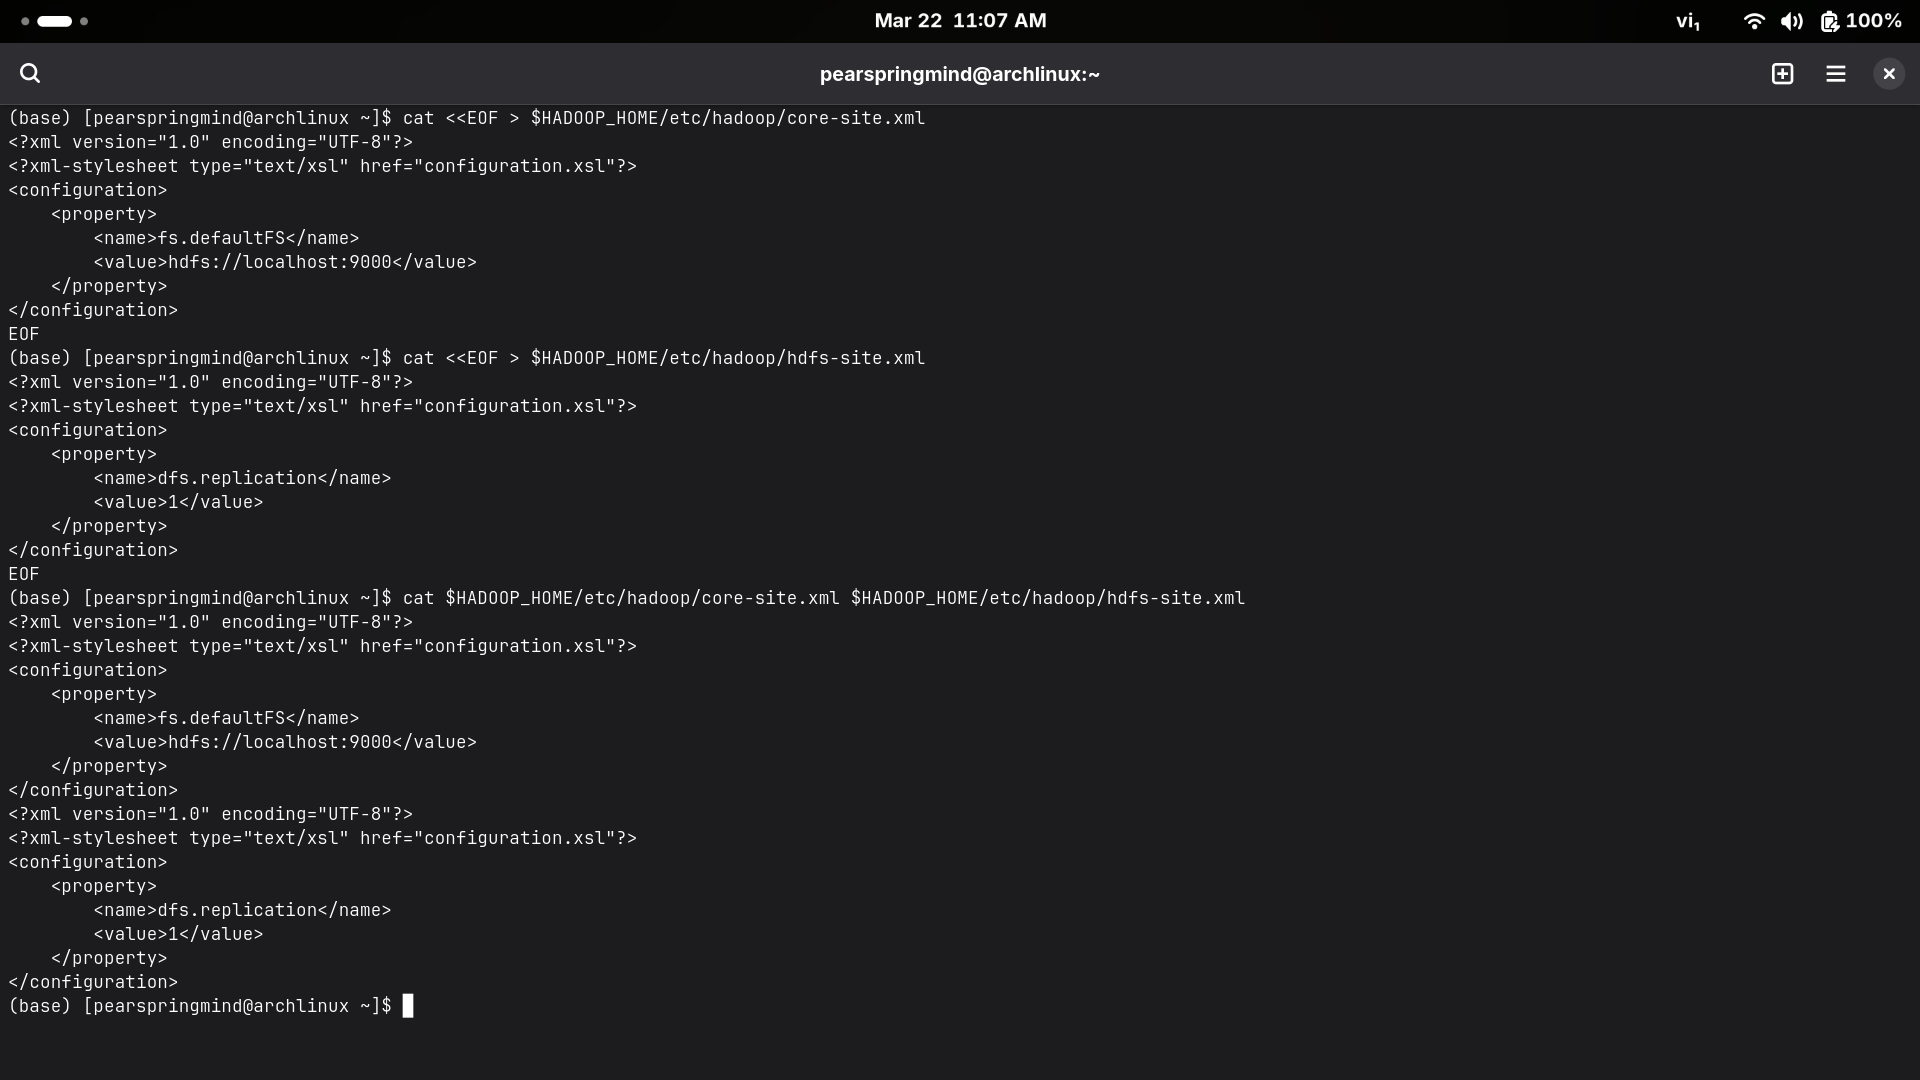
\includegraphics[width=\textwidth]{07-xml-config.png}
  \caption{Nội dung cấu hình core-site.xml và hdfs-site.xml}
  \label{fig:xml-config}
\end{figure}

% ------------------------------------------------------------
\subsection{Format NameNode}

Trước khi khởi động HDFS lần đầu tiên, NameNode cần được định dạng (format) để khởi
tạo cấu trúc thư mục metadata và tạo ID định danh cho cluster. Quá trình này tương
tự như định dạng một ổ đĩa cứng mới: nó xoá toàn bộ dữ liệu metadata cũ và tạo cấu
trúc mới từ đầu. Do đó, \textbf{không nên chạy lệnh format lại sau khi cluster đã
có dữ liệu}, vì điều này sẽ khiến DataNode không nhận ra cluster ID mới và toàn bộ
dữ liệu trên HDFS sẽ không còn truy cập được. Lệnh format chỉ nên thực hiện một lần
duy nhất khi cài đặt mới.

\begin{minted}{bash}
hdfs namenode -format
\end{minted}

\begin{figure}[H]
  \centering
  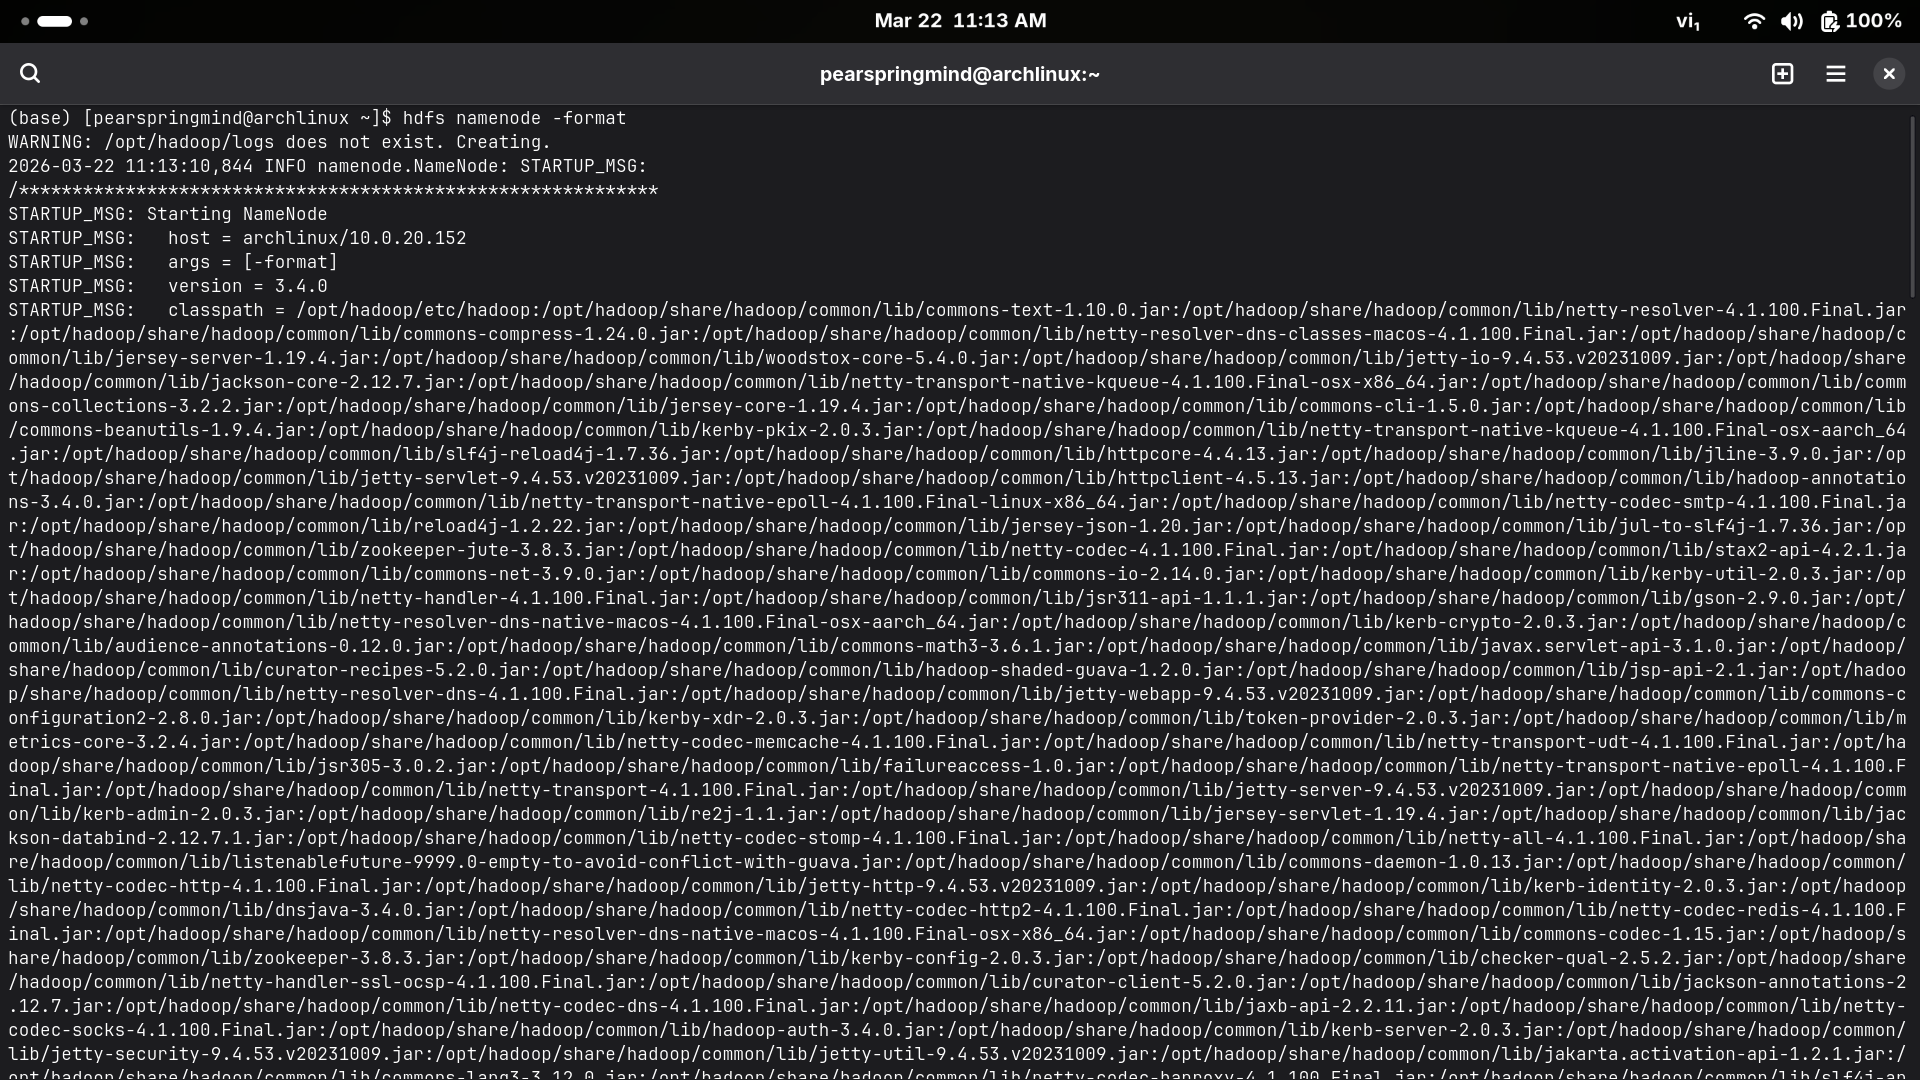
\includegraphics[width=\textwidth]{09-namenode-format.png}
  \caption{Format NameNode thành công — thông báo successfully formatted}
  \label{fig:namenode-format}
\end{figure}

% ------------------------------------------------------------
\subsection{Khởi động Cluster}

Sau khi format xong, tôi tiến hành khởi động cluster bằng hai script có sẵn trong
thư mục \texttt{sbin} của Hadoop. Script \texttt{start-dfs.sh} khởi động các tiến
trình liên quan đến hệ thống file phân tán: NameNode (quản lý metadata và namespace
của HDFS) và DataNode (lưu trữ dữ liệu thực tế theo dạng block). Script
\texttt{start-yarn.sh} khởi động ResourceManager (quản lý tài nguyên toàn cụm và
lên lịch các job) và NodeManager (quản lý tài nguyên trên từng node và thực thi
các container chứa task).

\begin{minted}{bash}
start-dfs.sh
start-yarn.sh
\end{minted}

\begin{figure}[H]
  \centering
  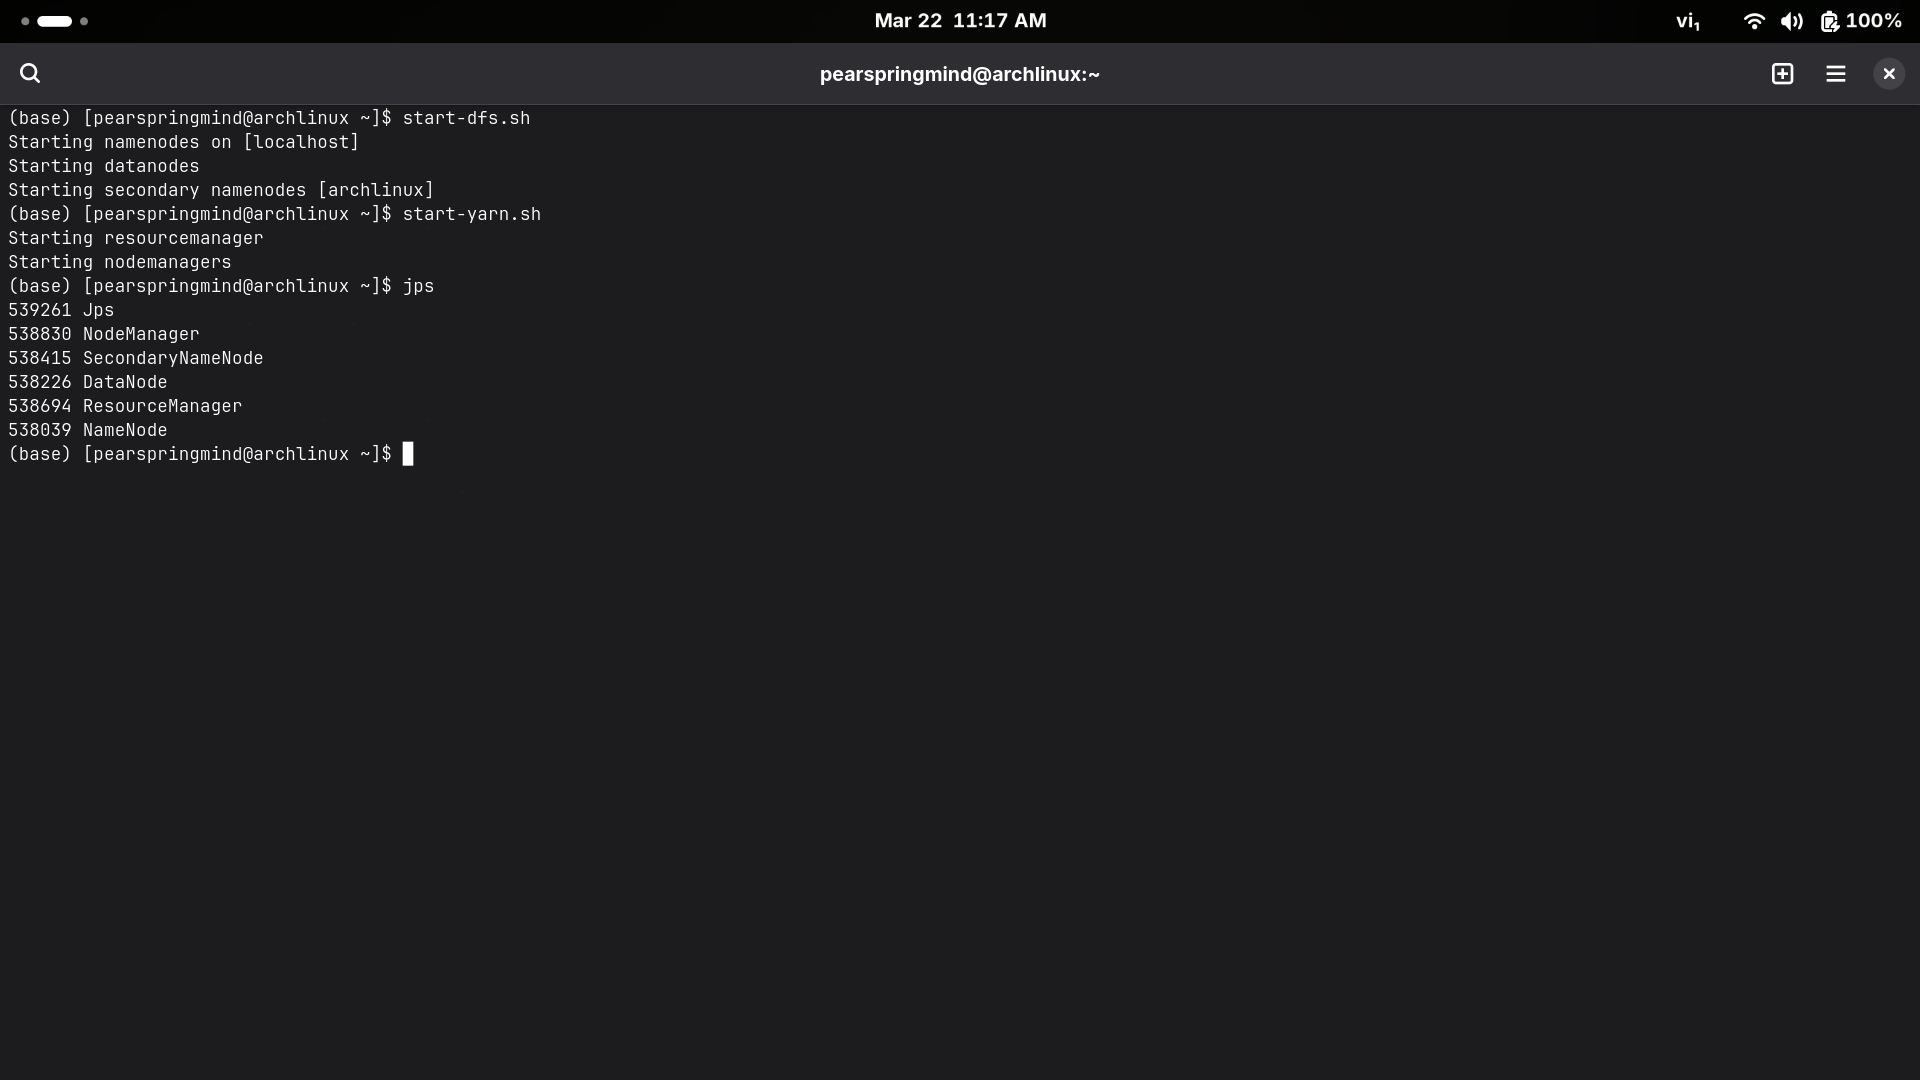
\includegraphics[width=\textwidth]{10-start-cluster-jps.png}
  \caption{Khởi động DFS, YARN và kiểm tra tiến trình JPS}
  \label{fig:start-cluster}
\end{figure}

% ------------------------------------------------------------
\subsection{Kiểm tra tiến trình (jps)}

Sau khi khởi động, tôi dùng lệnh \texttt{jps} (Java Virtual Machine Process Status
Tool) để liệt kê tất cả các tiến trình JVM đang chạy trên hệ thống. Trong chế độ
pseudo-distributed, cần có đủ 4 tiến trình daemon sau:
\begin{itemize}
  \item \textbf{NameNode} — quản lý namespace và metadata của HDFS;
  \item \textbf{DataNode} — lưu trữ các block dữ liệu thực tế;
  \item \textbf{ResourceManager} — quản lý và phân phối tài nguyên (CPU, RAM) trong
        cluster YARN;
  \item \textbf{NodeManager} — báo cáo tài nguyên và thực thi container trên node
        hiện tại.
\end{itemize}
Nếu thiếu bất kỳ tiến trình nào trong số này, cluster chưa hoạt động đúng và cần
kiểm tra log để xác định nguyên nhân.

\begin{minted}{bash}
jps
\end{minted}

\begin{figure}[H]
  \centering
  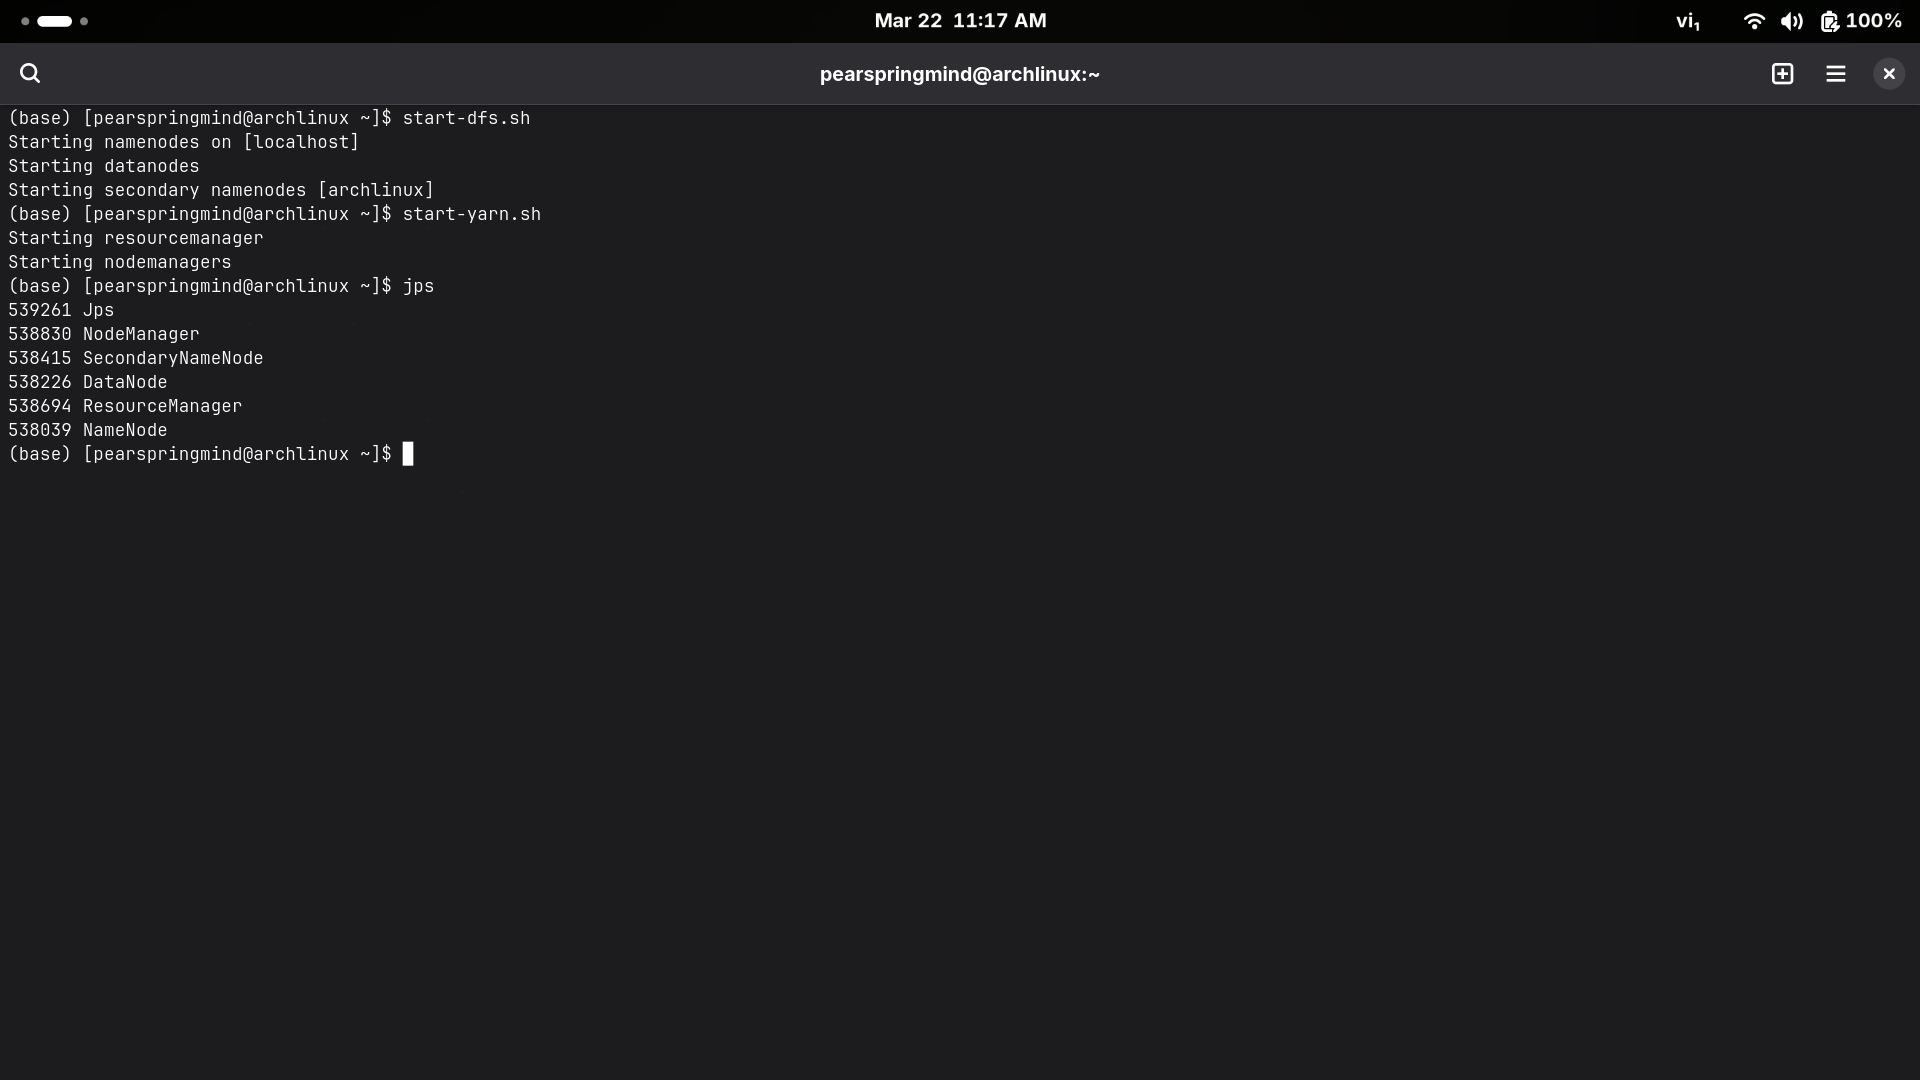
\includegraphics[width=\textwidth]{10-start-cluster-jps.png}
  \caption{Lệnh jps hiển thị đủ 4 tiến trình daemon}
  \label{fig:jps}
\end{figure}

% ------------------------------------------------------------
\subsection{WebUI — Giao diện quản trị}

Hadoop cung cấp giao diện web trực quan để giám sát trạng thái cluster mà không cần
dùng dòng lệnh. Tôi truy cập địa chỉ \url{http://localhost:9870} trên trình duyệt
để mở NameNode Web UI. Giao diện này cho phép xem thông tin tổng quan về cluster
như dung lượng HDFS đã dùng và còn trống, danh sách các DataNode đang hoạt động
(tab \textit{Datanodes}), cây thư mục HDFS (tab \textit{Utilities > Browse the file
system}), và nhật ký hoạt động. Việc tab \textit{Datanodes} hiển thị trạng thái
\textit{Live Nodes: 1} xác nhận DataNode đã kết nối thành công với NameNode.

\begin{figure}[H]
  \centering
  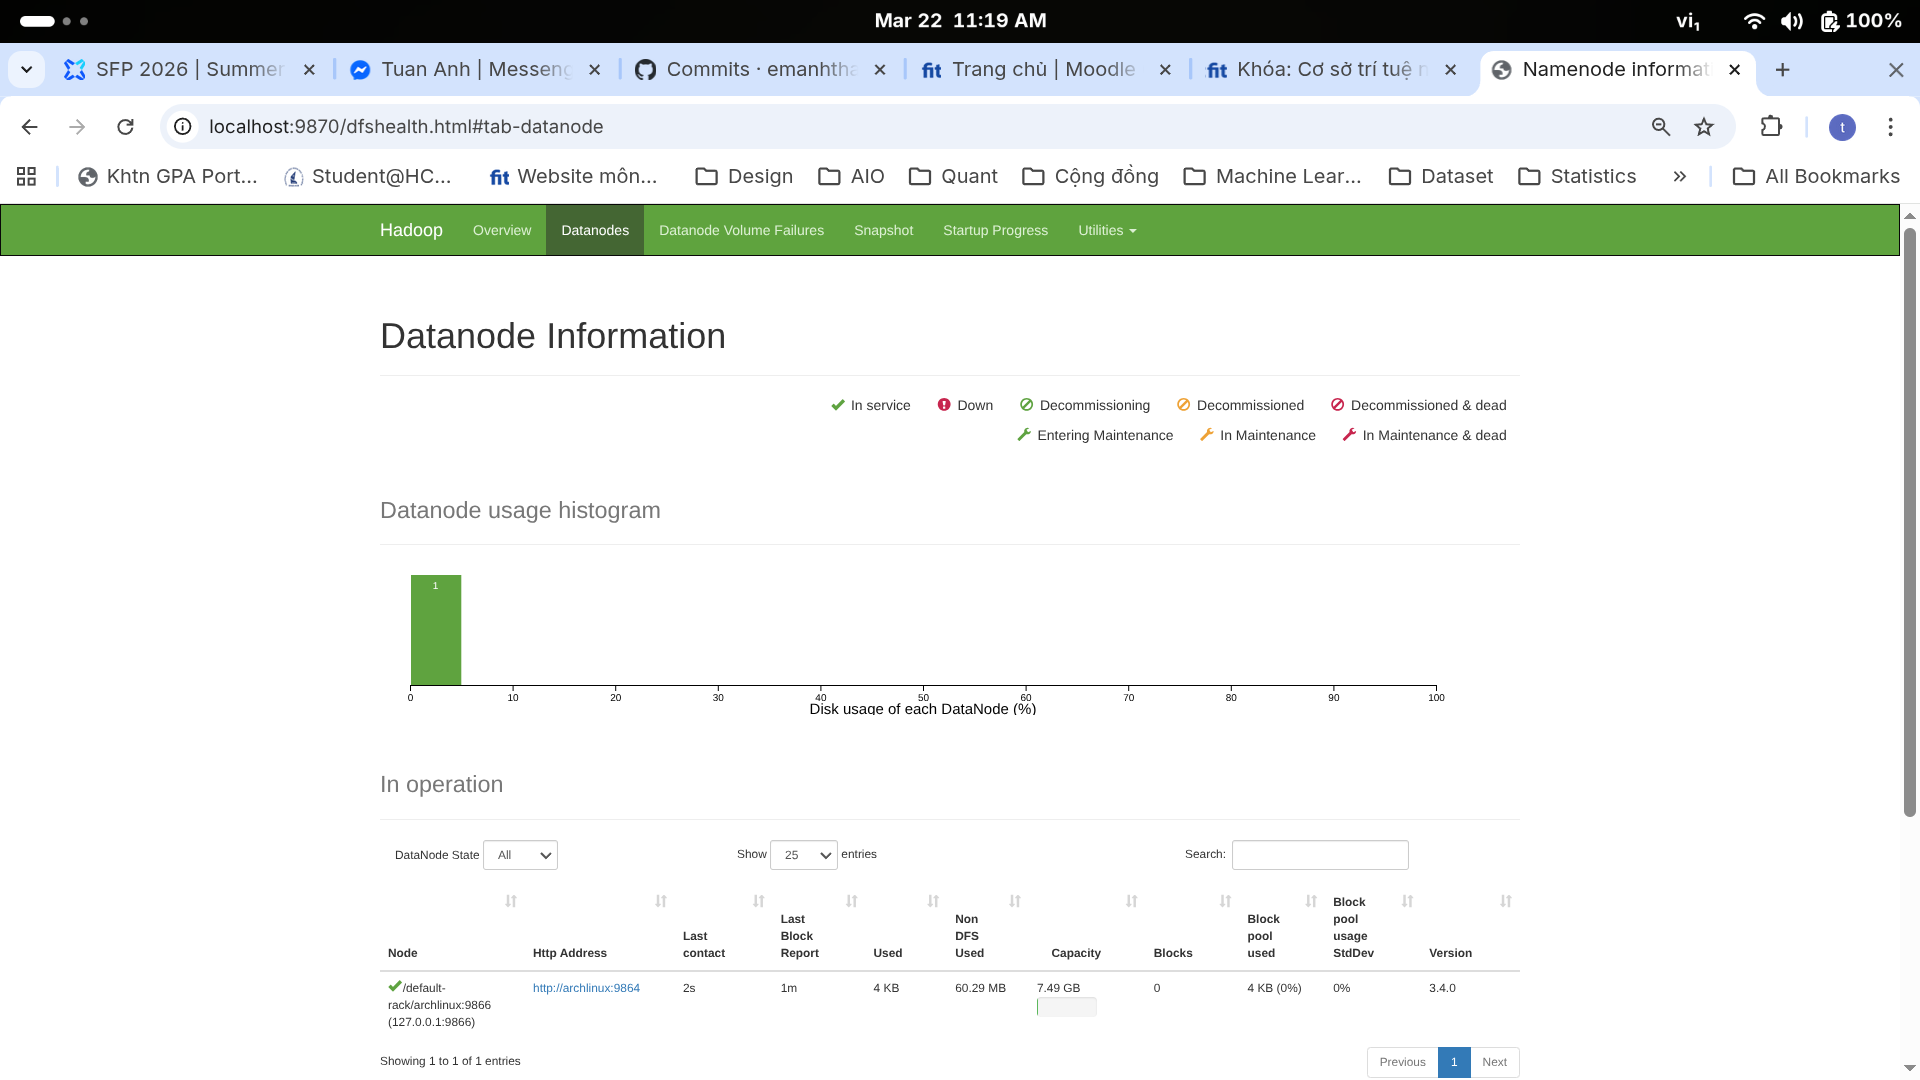
\includegraphics[width=0.85\textwidth]{11-webui-datanodes.png}
  \caption{Giao diện WebUI Hadoop — tab Datanodes hiển thị Live Nodes}
  \label{fig:webui}
\end{figure}

% ------------------------------------------------------------
\subsection{Tạo thư mục HDFS và User}

Theo yêu cầu của bài lab, tôi tạo cấu trúc thư mục trên HDFS phục vụ cho việc lưu
trữ dữ liệu theo từng sinh viên. Thư mục gốc \texttt{/hcmus} được tạo để chứa dữ
liệu của tất cả thành viên, sau đó thư mục con \texttt{/hcmus/23120099} được tạo
riêng cho MSSV của tôi. Song song với việc tạo thư mục HDFS, tôi tạo tài khoản
Linux mới \texttt{khtn\_23120099} để phục vụ bước phân quyền ở mục tiếp theo; tài
khoản này sẽ được gán làm chủ sở hữu (owner) của thư mục HDFS tương ứng.

\begin{minted}{bash}
hdfs dfs -mkdir /hcmus
sudo useradd -m khtn_23120099
hdfs dfs -mkdir /hcmus/23120099
\end{minted}

\begin{figure}[H]
  \centering
  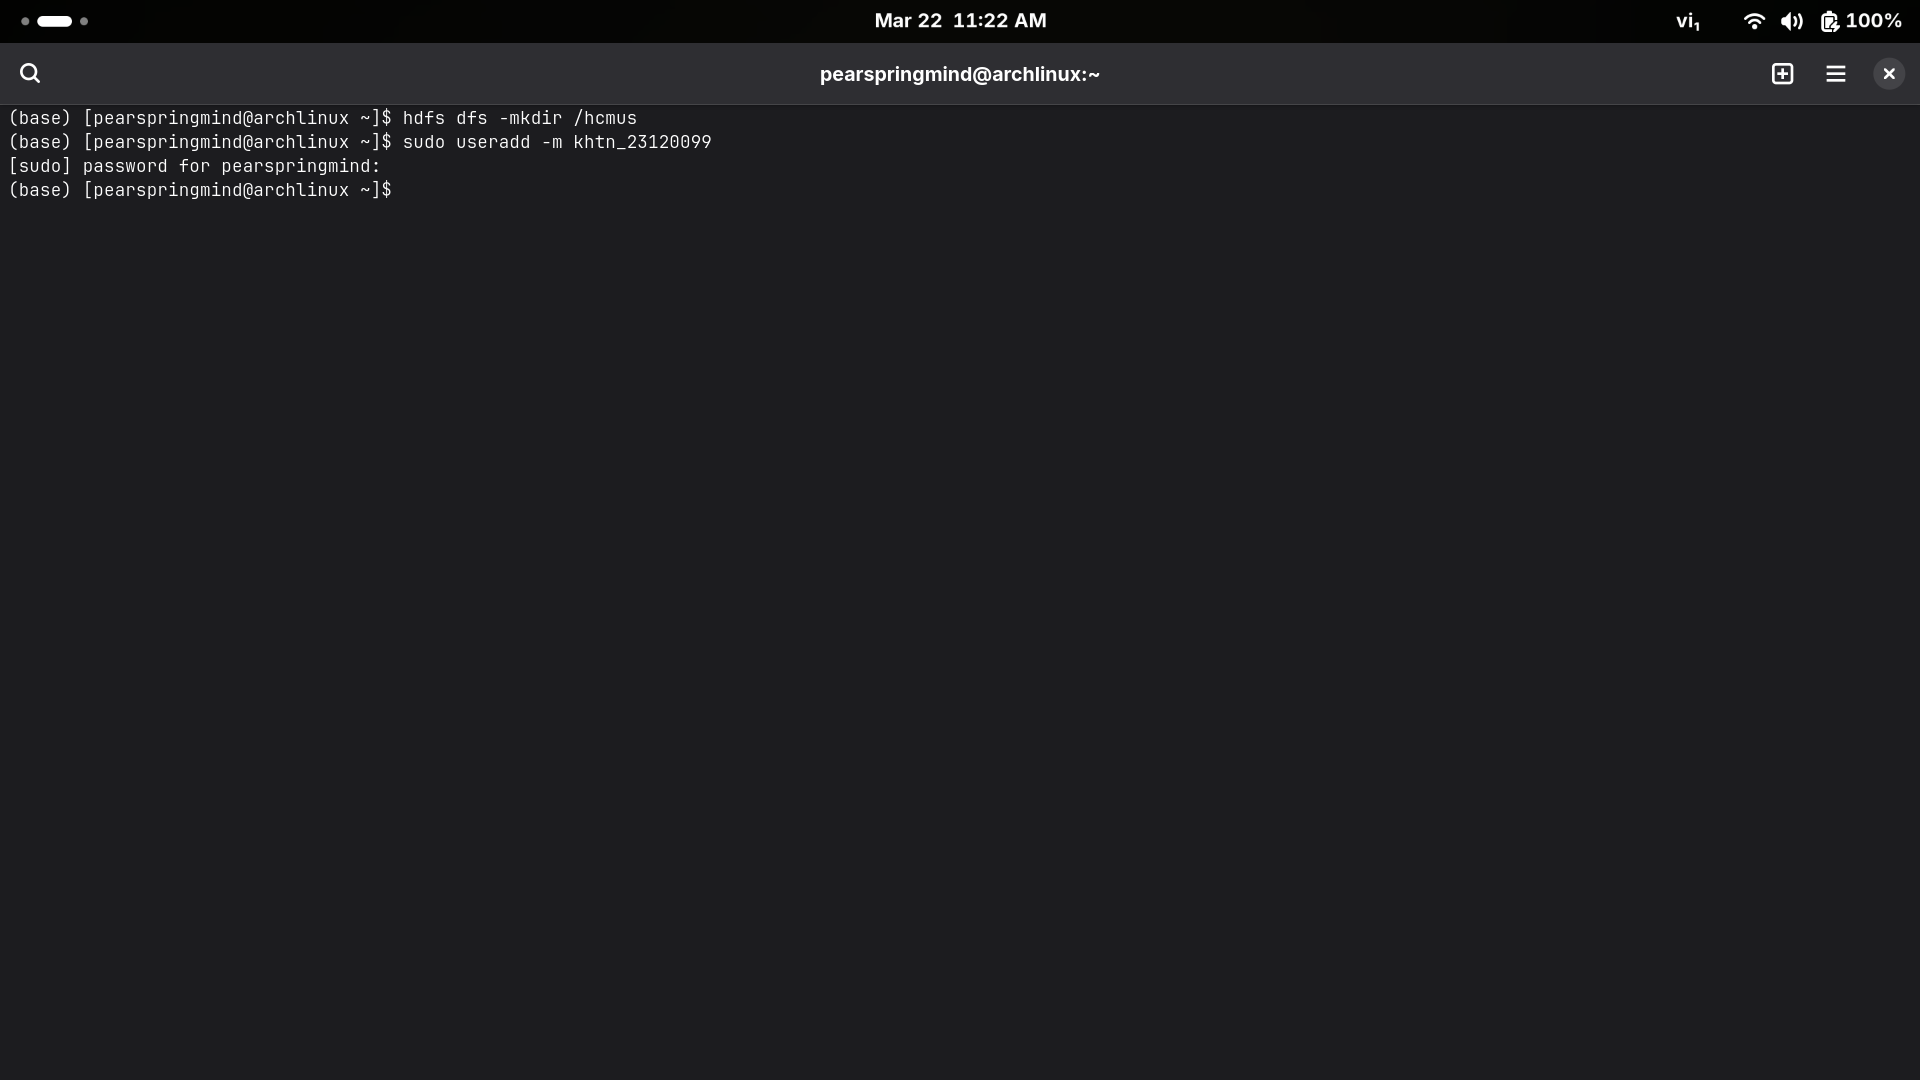
\includegraphics[width=0.48\textwidth]{12-hdfs-mkdir-user.png}
  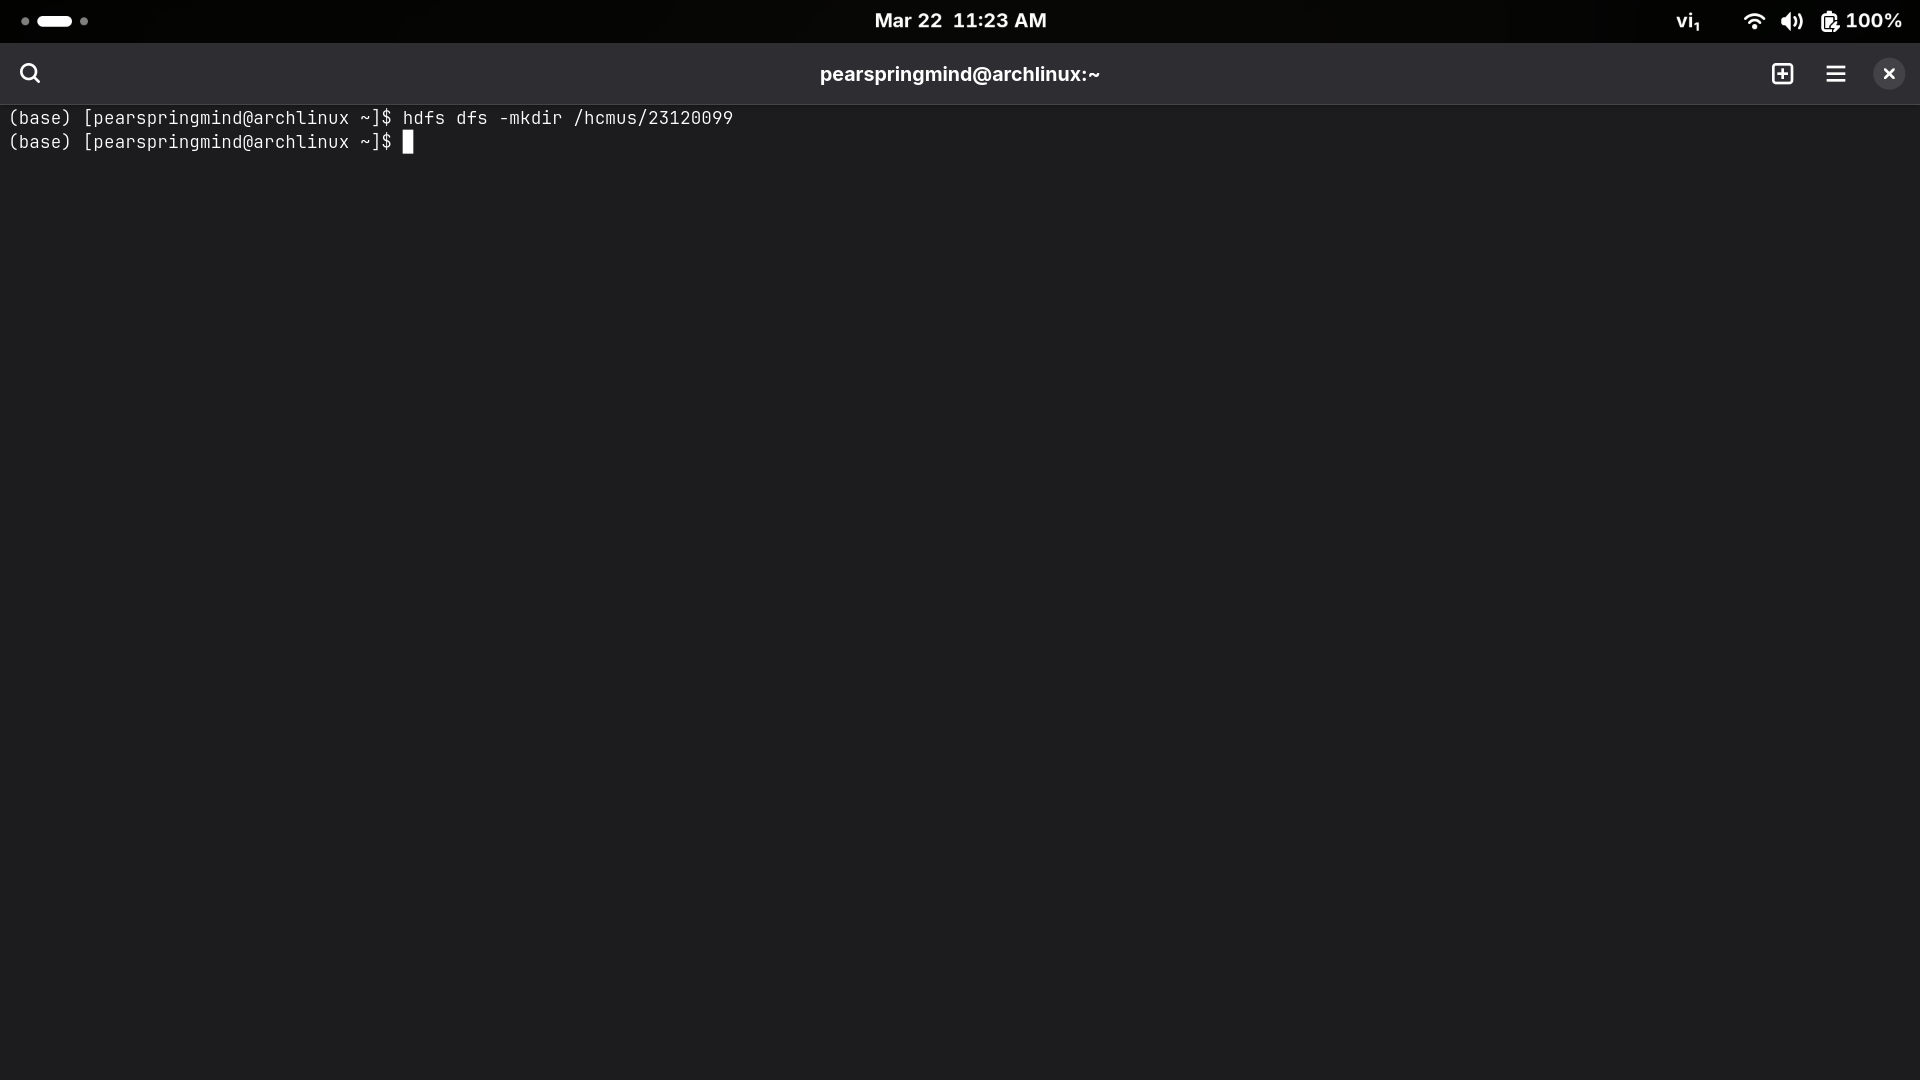
\includegraphics[width=0.48\textwidth]{13-hdfs-mkdir-sub.png}
  \caption{Tạo thư mục HDFS /hcmus/23120099 và user Linux khtn\_23120099}
  \label{fig:mkdir-user}
\end{figure}

% ------------------------------------------------------------
\subsection{Tải dữ liệu lên HDFS}

Tôi tải file \texttt{words.txt} — danh sách từ dùng cho bài toán WordCount — lên
thư mục HDFS đã tạo bằng lệnh \texttt{hdfs dfs -put}. Lệnh này sao chép file từ hệ
thống file cục bộ lên HDFS, phân chia thành các block (mặc định 128 MB) và phân
phối đến các DataNode theo chính sách replication đã cấu hình. Sau khi tải lên, tôi
xác nhận file đã tồn tại trên HDFS bằng lệnh \texttt{-ls}, kiểm tra kích thước
và thời gian sửa đổi để đảm bảo dữ liệu được tải lên đầy đủ.

\begin{minted}{bash}
hdfs dfs -put words.txt /hcmus/23120099/
hdfs dfs -ls /hcmus/23120099/
\end{minted}

\begin{figure}[H]
  \centering
  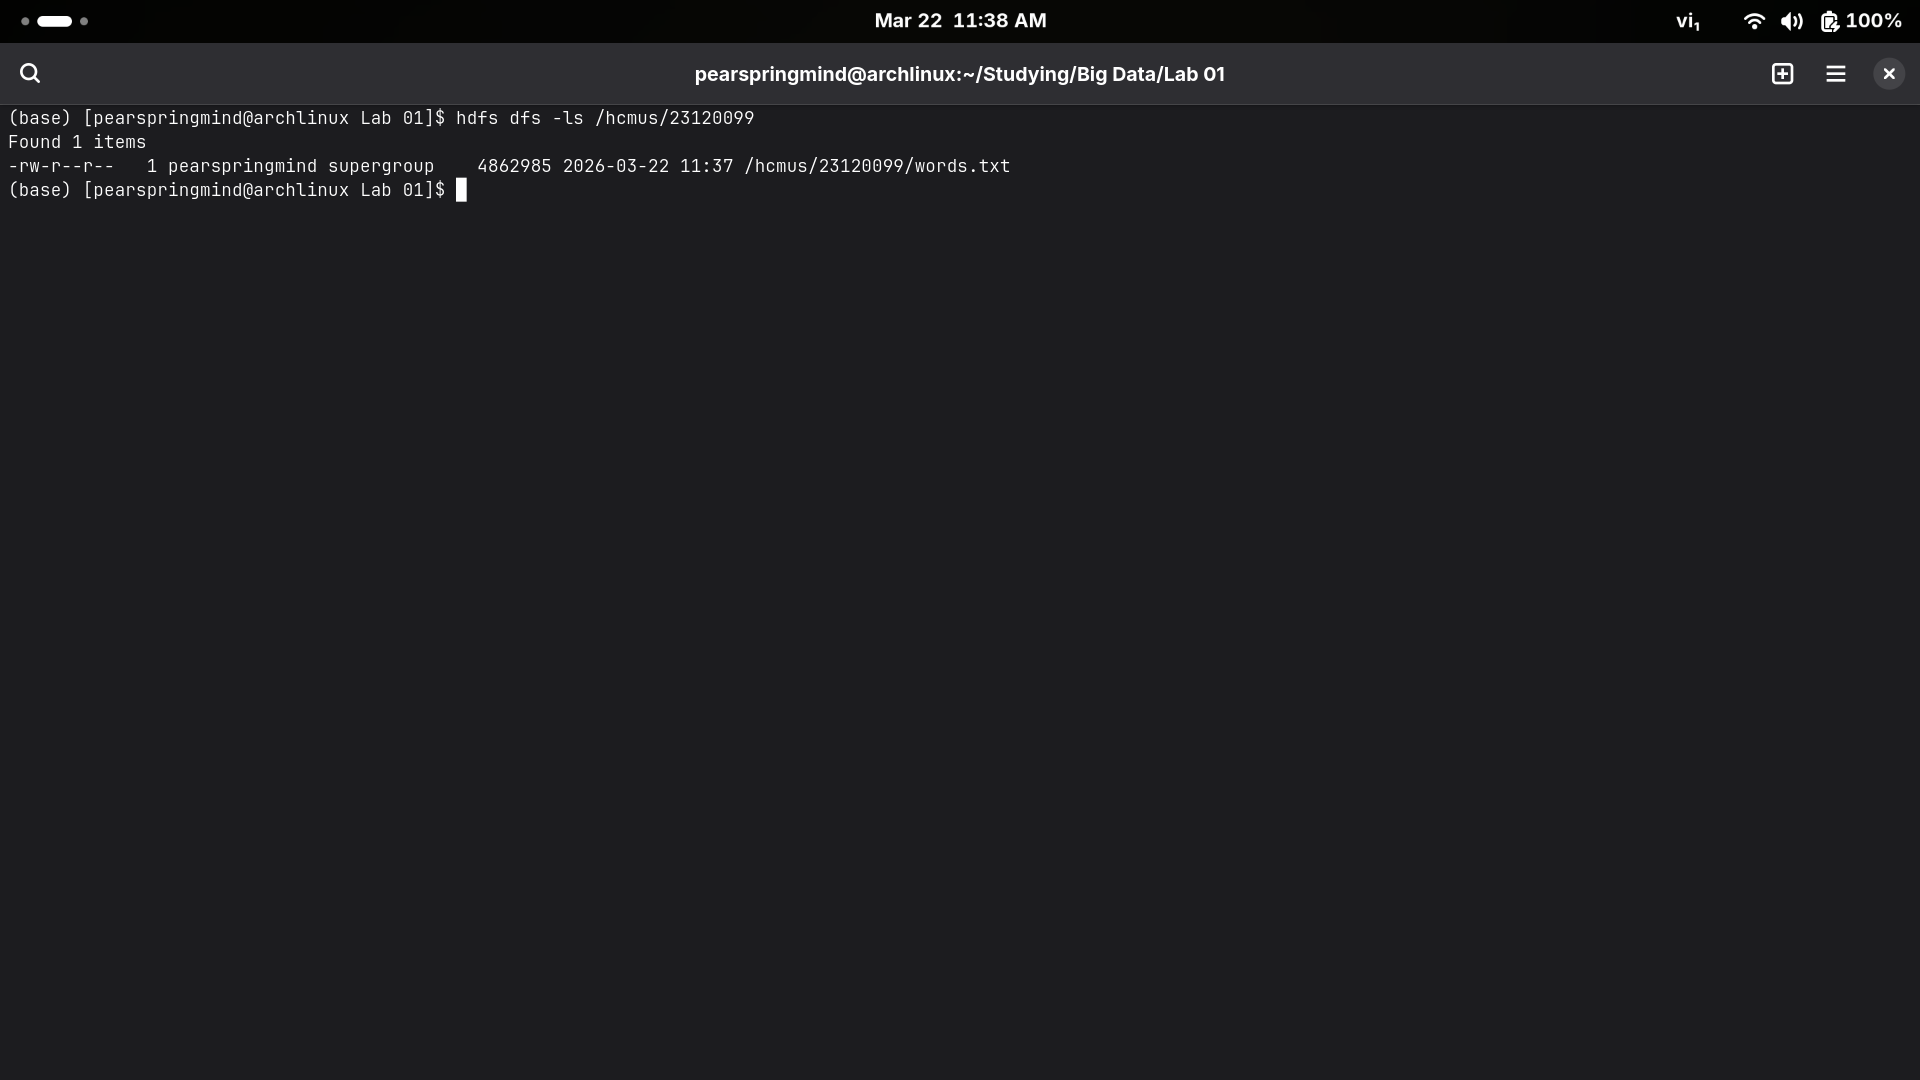
\includegraphics[width=\textwidth]{14-hdfs-put-confirm.png}
  \caption{Tải file words.txt lên HDFS và xác nhận bằng lệnh ls}
  \label{fig:hdfs-put}
\end{figure}

% ------------------------------------------------------------
\subsection{Phân quyền và chuyển Owner}

Để đảm bảo bảo mật và tuân thủ mô hình phân quyền của HDFS, tôi thực hiện hai thao
tác: đặt quyền truy cập theo chuẩn Unix octal \texttt{744} (nghĩa là chủ sở hữu có
toàn quyền đọc-ghi-thực thi \texttt{rwx}, còn nhóm và người khác chỉ có quyền đọc
\texttt{r--}), và chuyển quyền sở hữu thư mục sang tài khoản \texttt{khtn\_23120099}
đã tạo trước đó. Lệnh \texttt{-ls /hcmus/} sau đó xác nhận thông tin phân quyền và
owner đã được áp dụng đúng.

\begin{minted}{bash}
hdfs dfs -chmod 744 /hcmus/23120099
hdfs dfs -chown khtn_23120099 /hcmus/23120099
hdfs dfs -ls /hcmus/
\end{minted}

\begin{figure}[H]
  \centering
  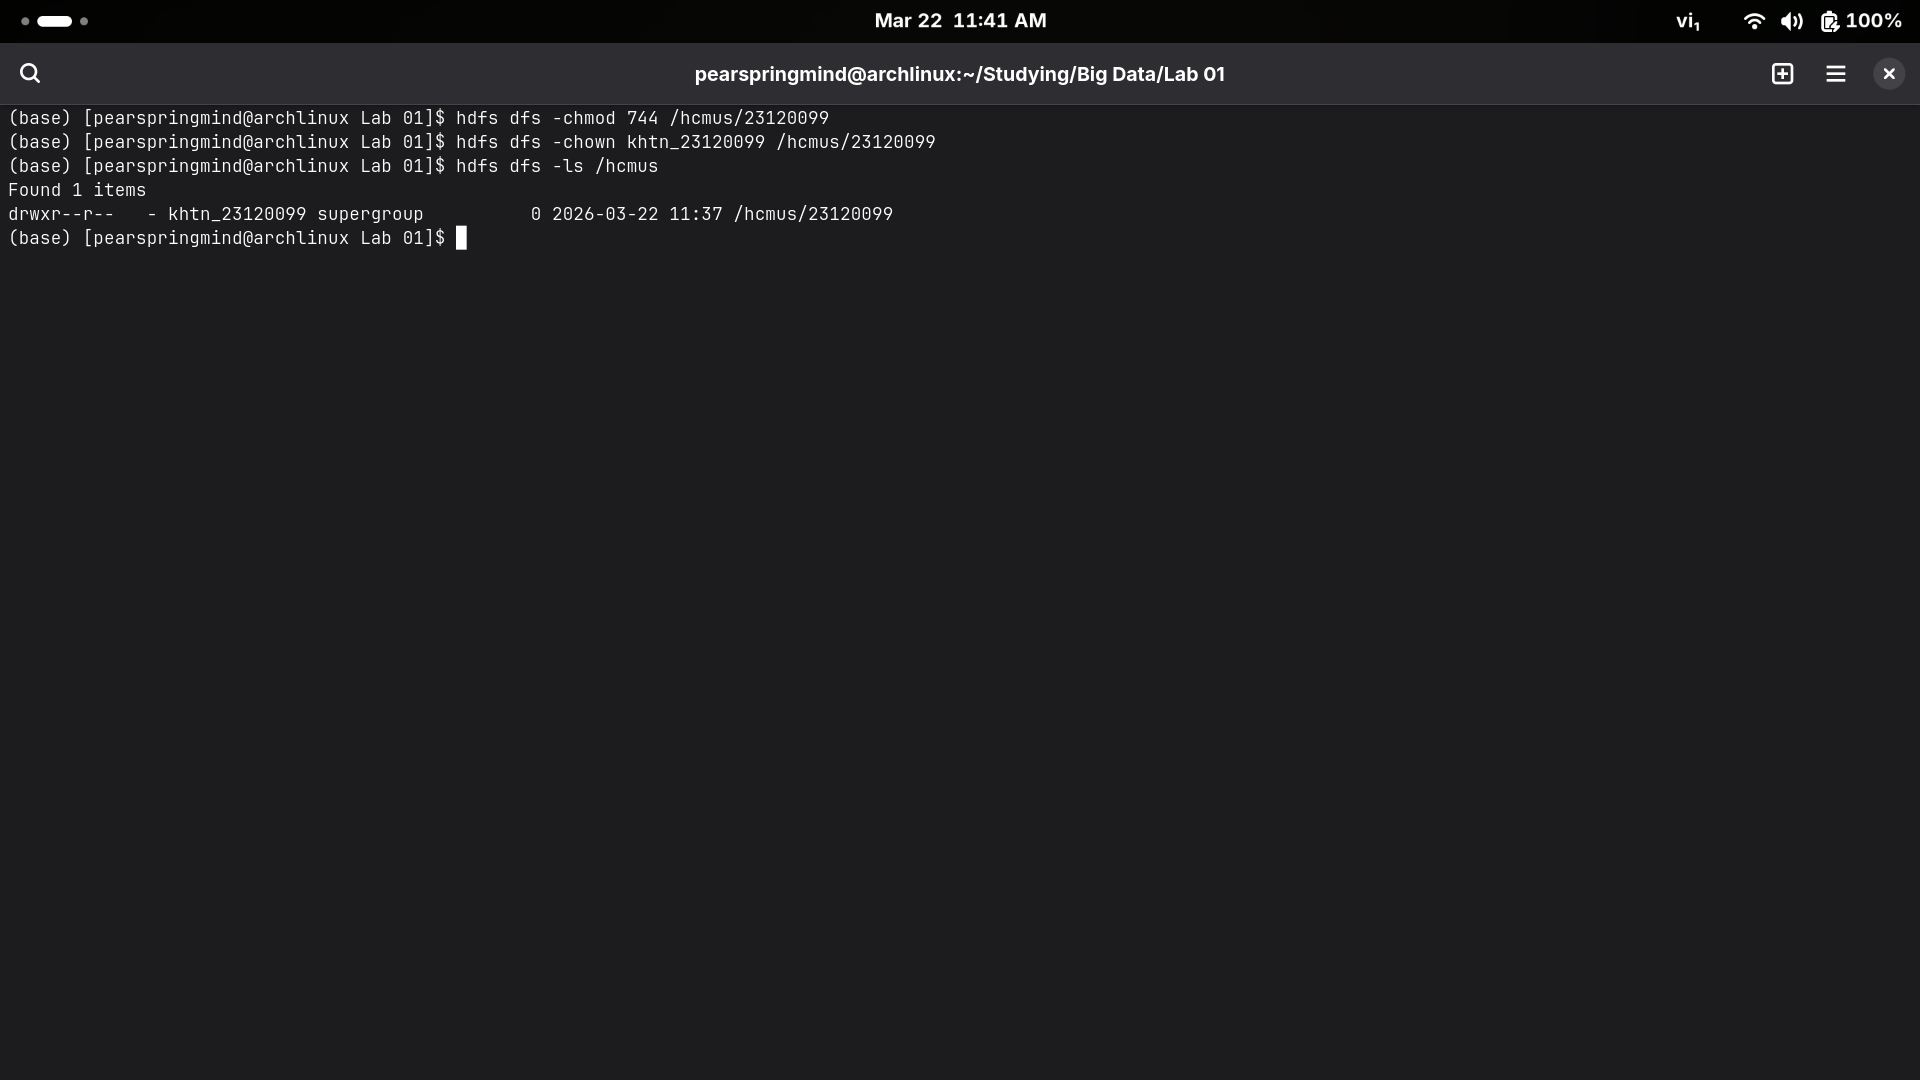
\includegraphics[width=\textwidth]{15-hdfs-chmod-chown.png}
  \caption{Phân quyền chmod 744 và chuyển owner cho khtn\_23120099}
  \label{fig:chmod-chown}
\end{figure}

% ------------------------------------------------------------
\subsection{Chạy file JAR xác thực}

File \texttt{hadoop-test.jar} là công cụ xác thực do giáo viên cung cấp, có nhiệm
vụ kết nối vào HDFS thông qua cổng đã cấu hình, đọc thông tin thư mục của sinh viên,
ghi nhận địa chỉ MAC của máy đang chạy, và tạo ra file kết quả \texttt{23120099\_verification.txt}
chứa thông tin xác thực duy nhất. File kết quả này dùng để chứng minh rằng sinh viên
đã thực sự cài đặt và vận hành Hadoop thành công trên máy của mình, không phải copy
kết quả từ người khác.

\begin{minted}{bash}
java -jar hadoop-test.jar 9000 /hcmus/23120099
cat 23120099_verification.txt
\end{minted}

Nội dung file xác thực \texttt{23120099\_verification.txt} thu được sau khi chạy JAR:

\begin{minted}{text}
MAC=14-5A-FC-90-C5-E7
8a656a9128bc02d0e9668d65b0c0a4e0951c1024deee63891fec5a6c2015a943
\end{minted}

\begin{figure}[H]
  \centering
  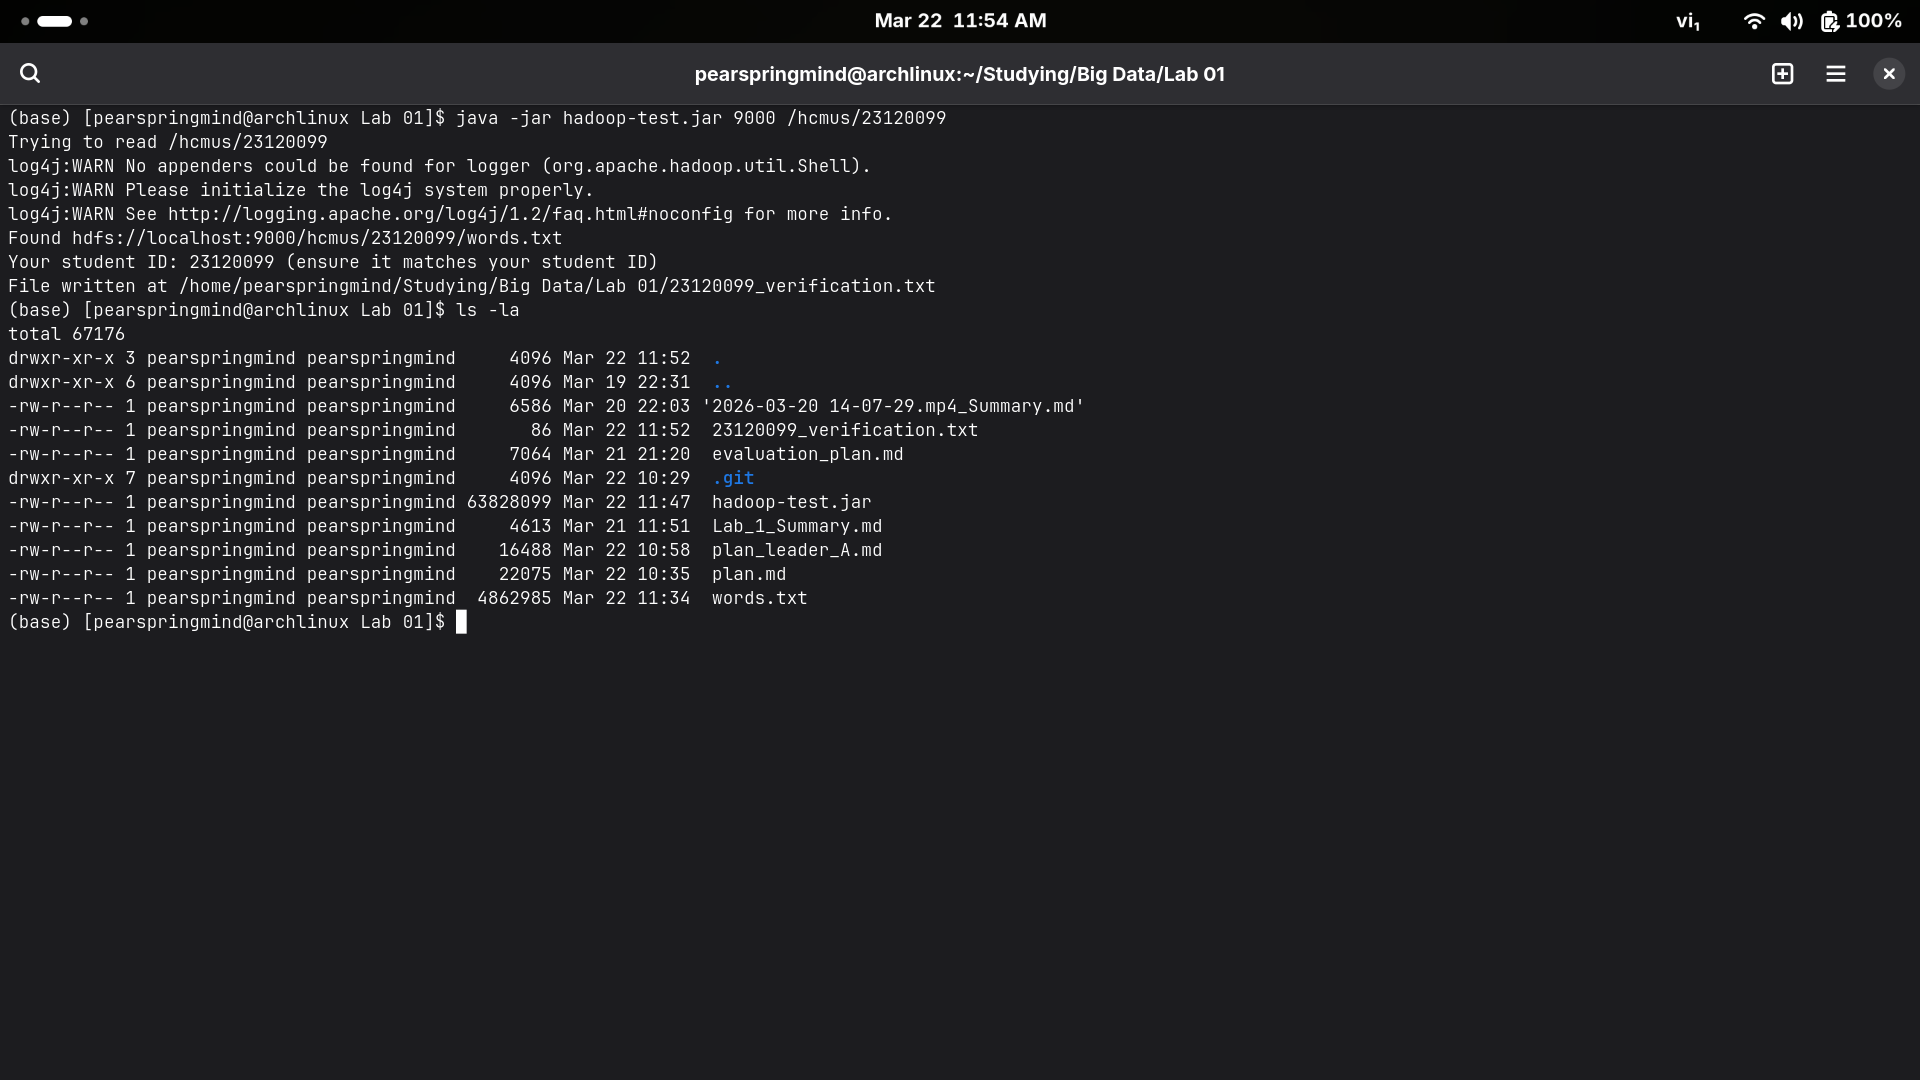
\includegraphics[width=\textwidth]{16-jar-verification.png}
  \caption{Chạy hadoop-test.jar và tạo file xác thực minh chứng thành công}
  \label{fig:jar-run}
\end{figure}

\begin{figure}[H]
  \centering
  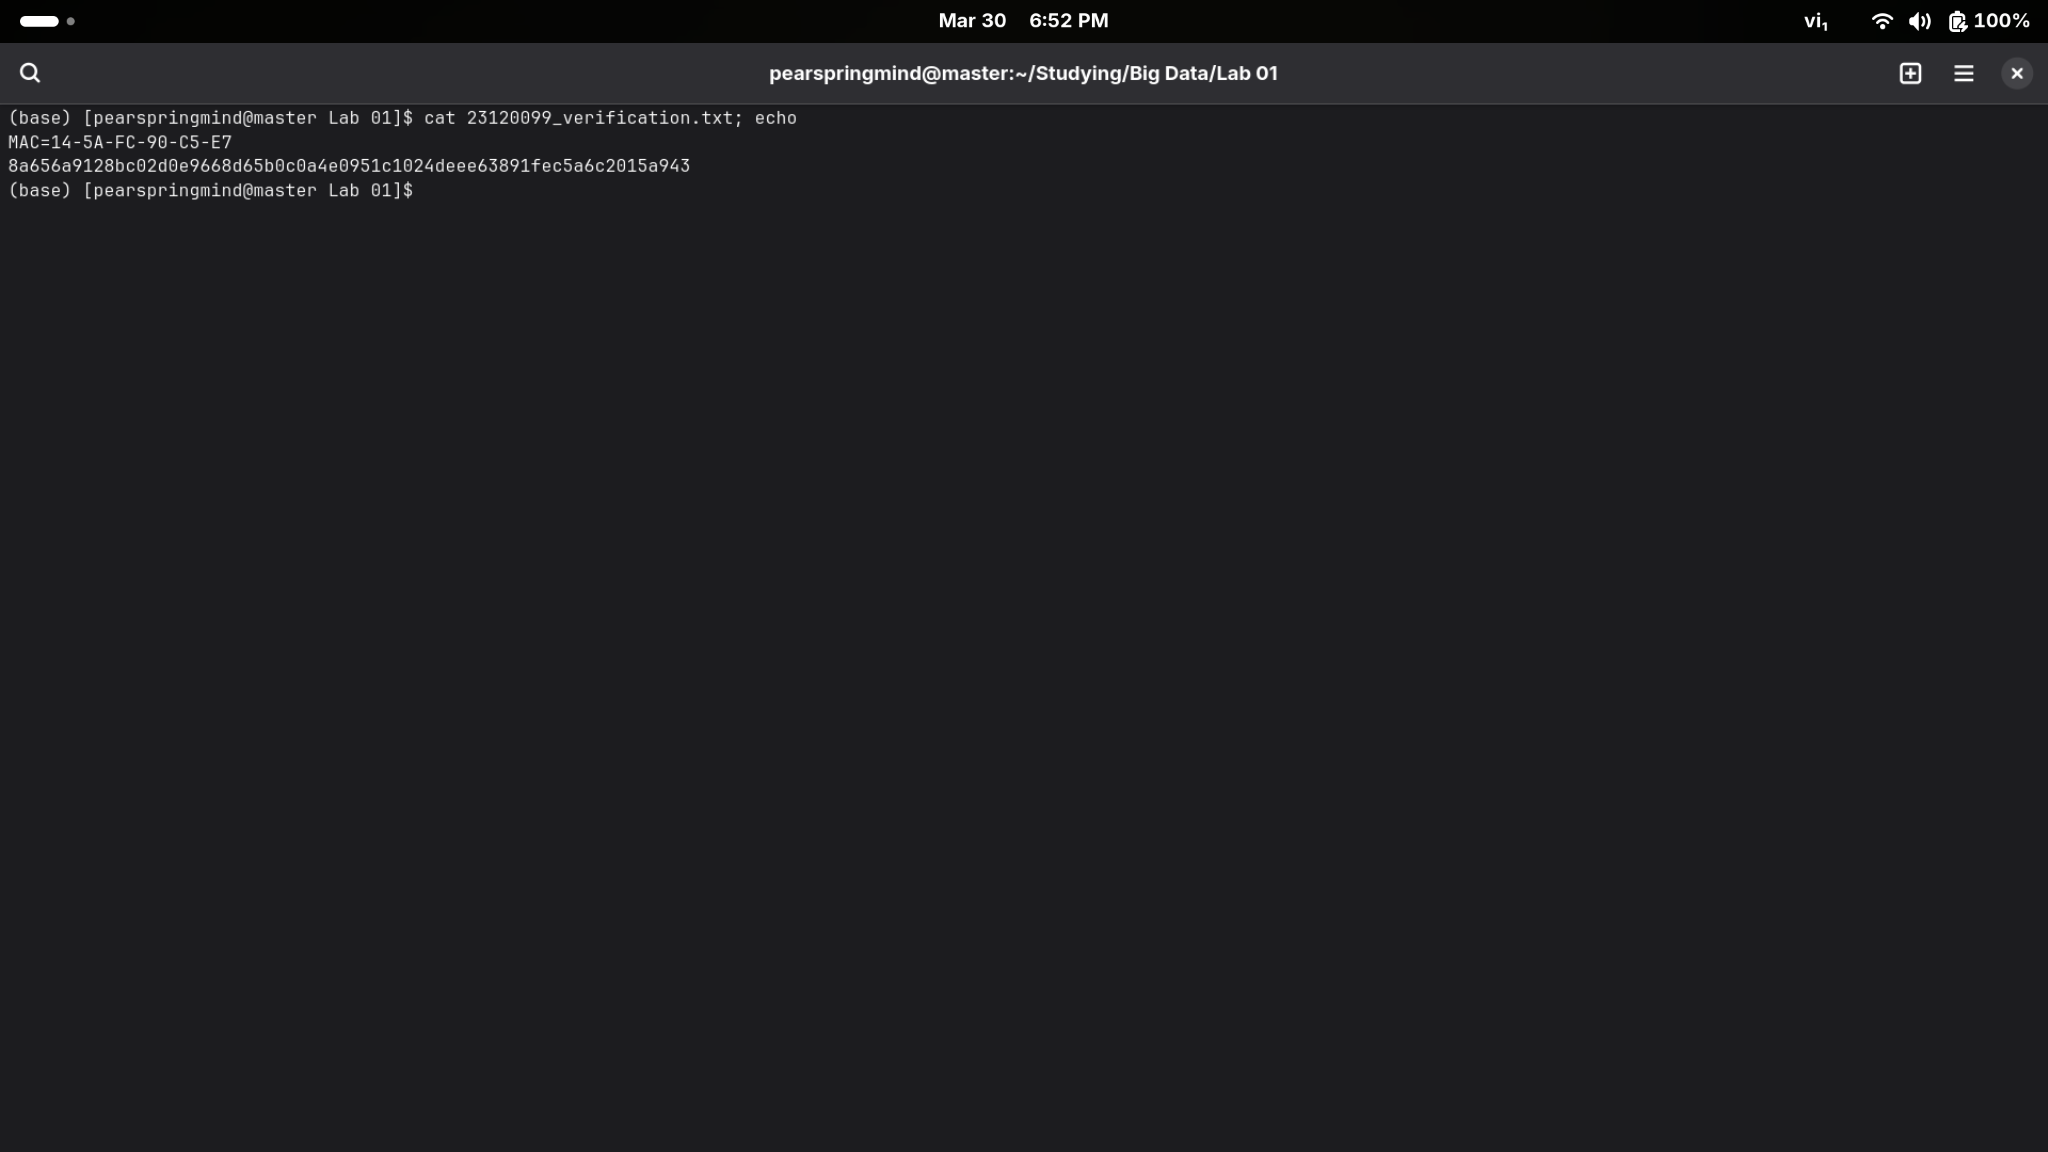
\includegraphics[width=\textwidth]{verification-txt.png}
  \caption{Nội dung file 23120099\_verification.txt}
  \label{fig:verification}
\end{figure}

% ------------------------------------------------------------
\subsection{Xử lý sự cố rủi ro môi trường do Incompatible ClusterID}

Trong quá trình vận hành, do tác động của việc format lại cấu trúc NameNode bằng lệnh \texttt{hdfs namenode -format} nhiều lần, NameNode đã sinh ra ClusterID mới. Trong lúc đó, thư mục dữ liệu của DataNode (\texttt{/opt/hadoop/data/datanode}) vẫn còn lưu ClusterID cũ từ lần chạy trước. Hệ quả là DataNode từ chối kết nối và ngưng hoạt động với thông báo lỗi \texttt{java.io.IOException: Incompatible clusterIDs}.

\begin{figure}[H]
  \centering
  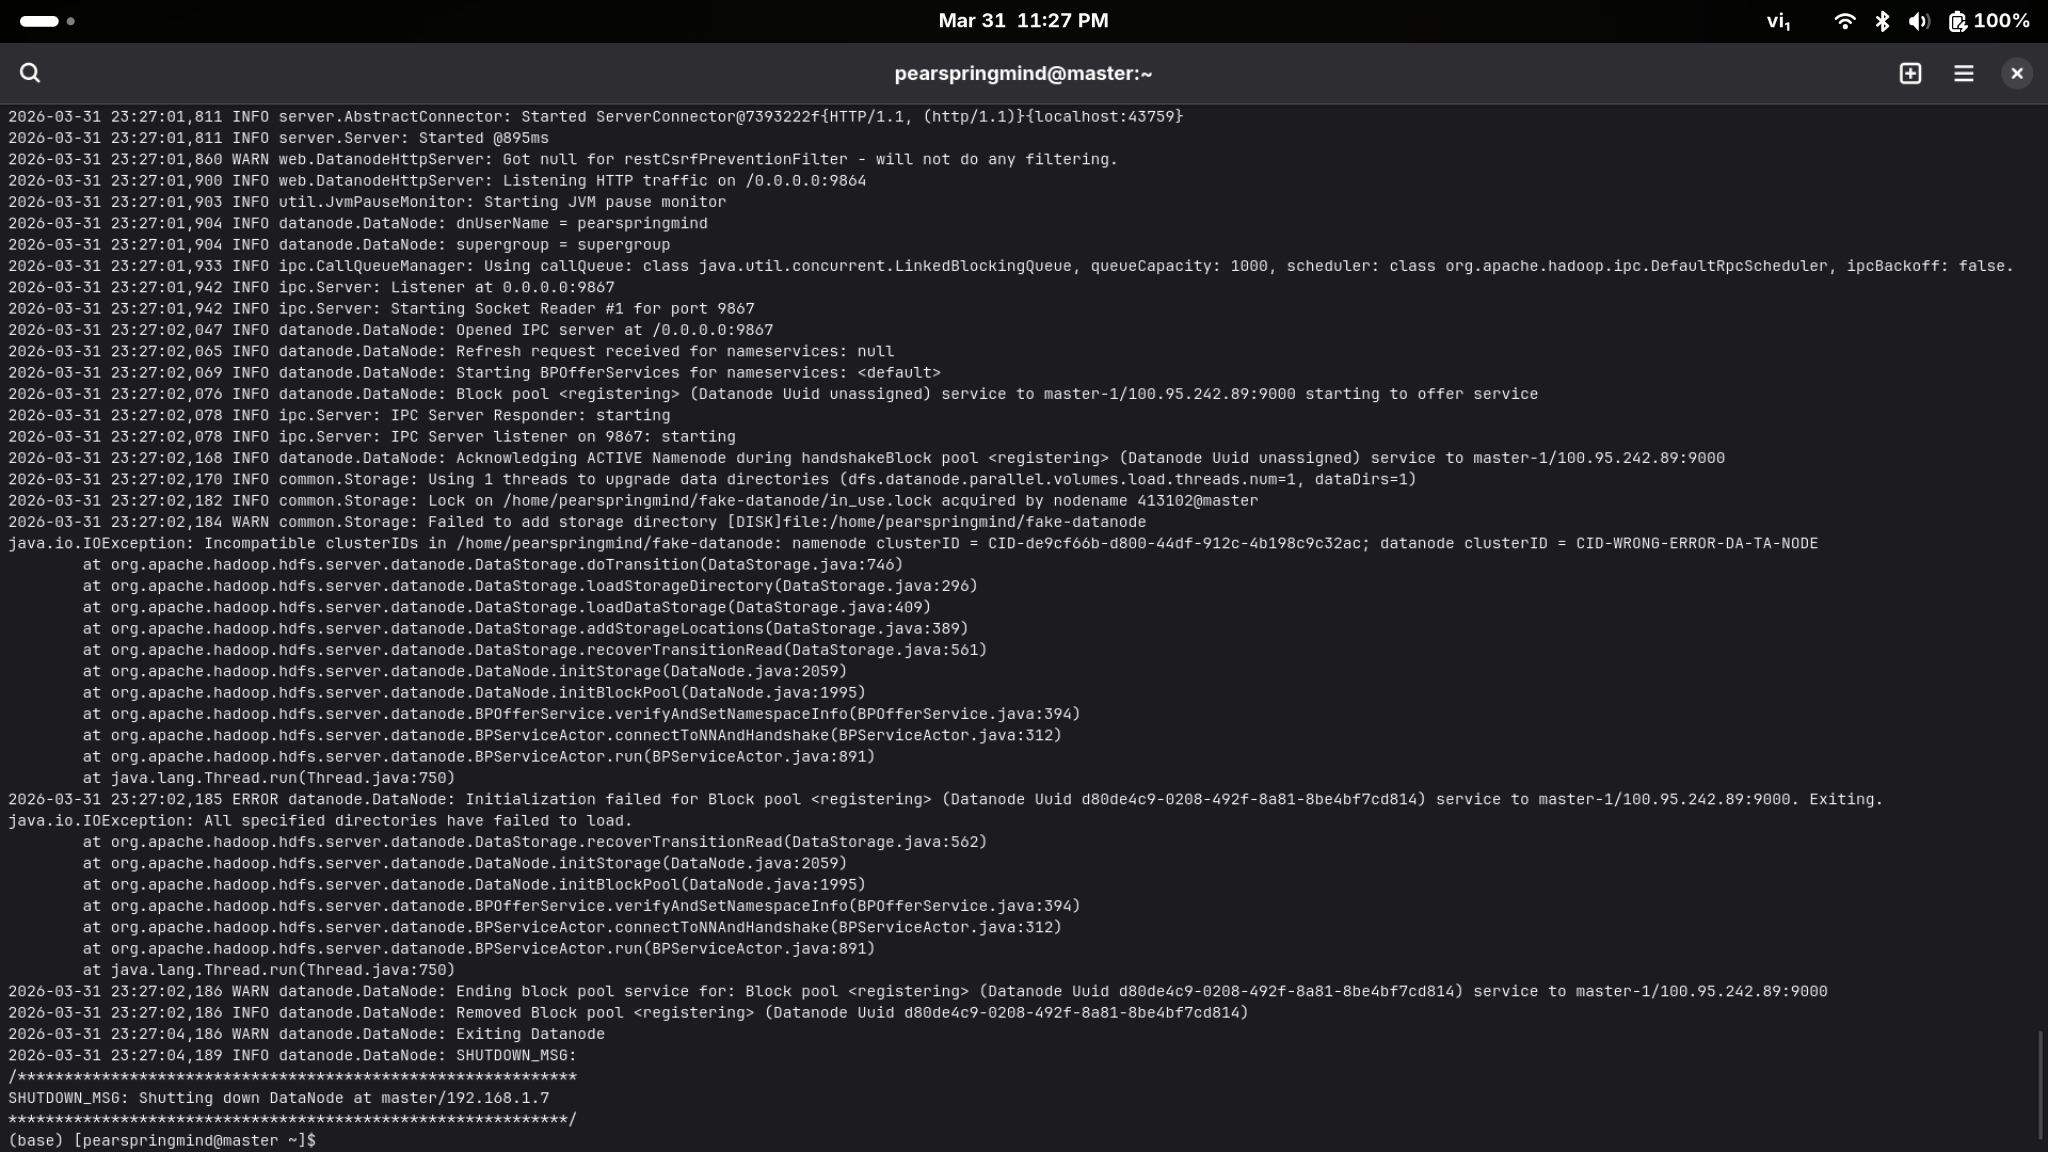
\includegraphics[width=\textwidth]{error-clusterid.png}
  \caption{Lỗi Incompatible clusterIDs khiến DataNode không thể hoạt động do xung đột ID}
  \label{fig:error-clusterid}
\end{figure}

Theo hướng dẫn tra cứu trên cộng đồng lập trình viên StackOverflow về vấn đề cấu hình HDFS (Hình \ref{fig:troubleshoot-search}), tôi đã tiến hành xử lý triệt để như sau:
\begin{itemize}
    \item Dừng toàn bộ hệ thống bằng lệnh \texttt{stop-dfs.sh} và \texttt{stop-yarn.sh}.
    \item Xoá sạch thư mục dữ liệu DataNode bị xung đột thông qua lệnh \texttt{rm -rf /opt/hadoop/data/datanode} (do trên môi trường mới chưa lưu trữ file dữ liệu nào quan trọng).
    \item Tiến hành khởi động lại bằng \texttt{start-dfs.sh}. Lúc này, quá trình DataNode bootstrap sẽ tự động đồng bộ lại ClusterID mới nhất từ NameNode.
\end{itemize}

\begin{figure}[H]
  \centering
  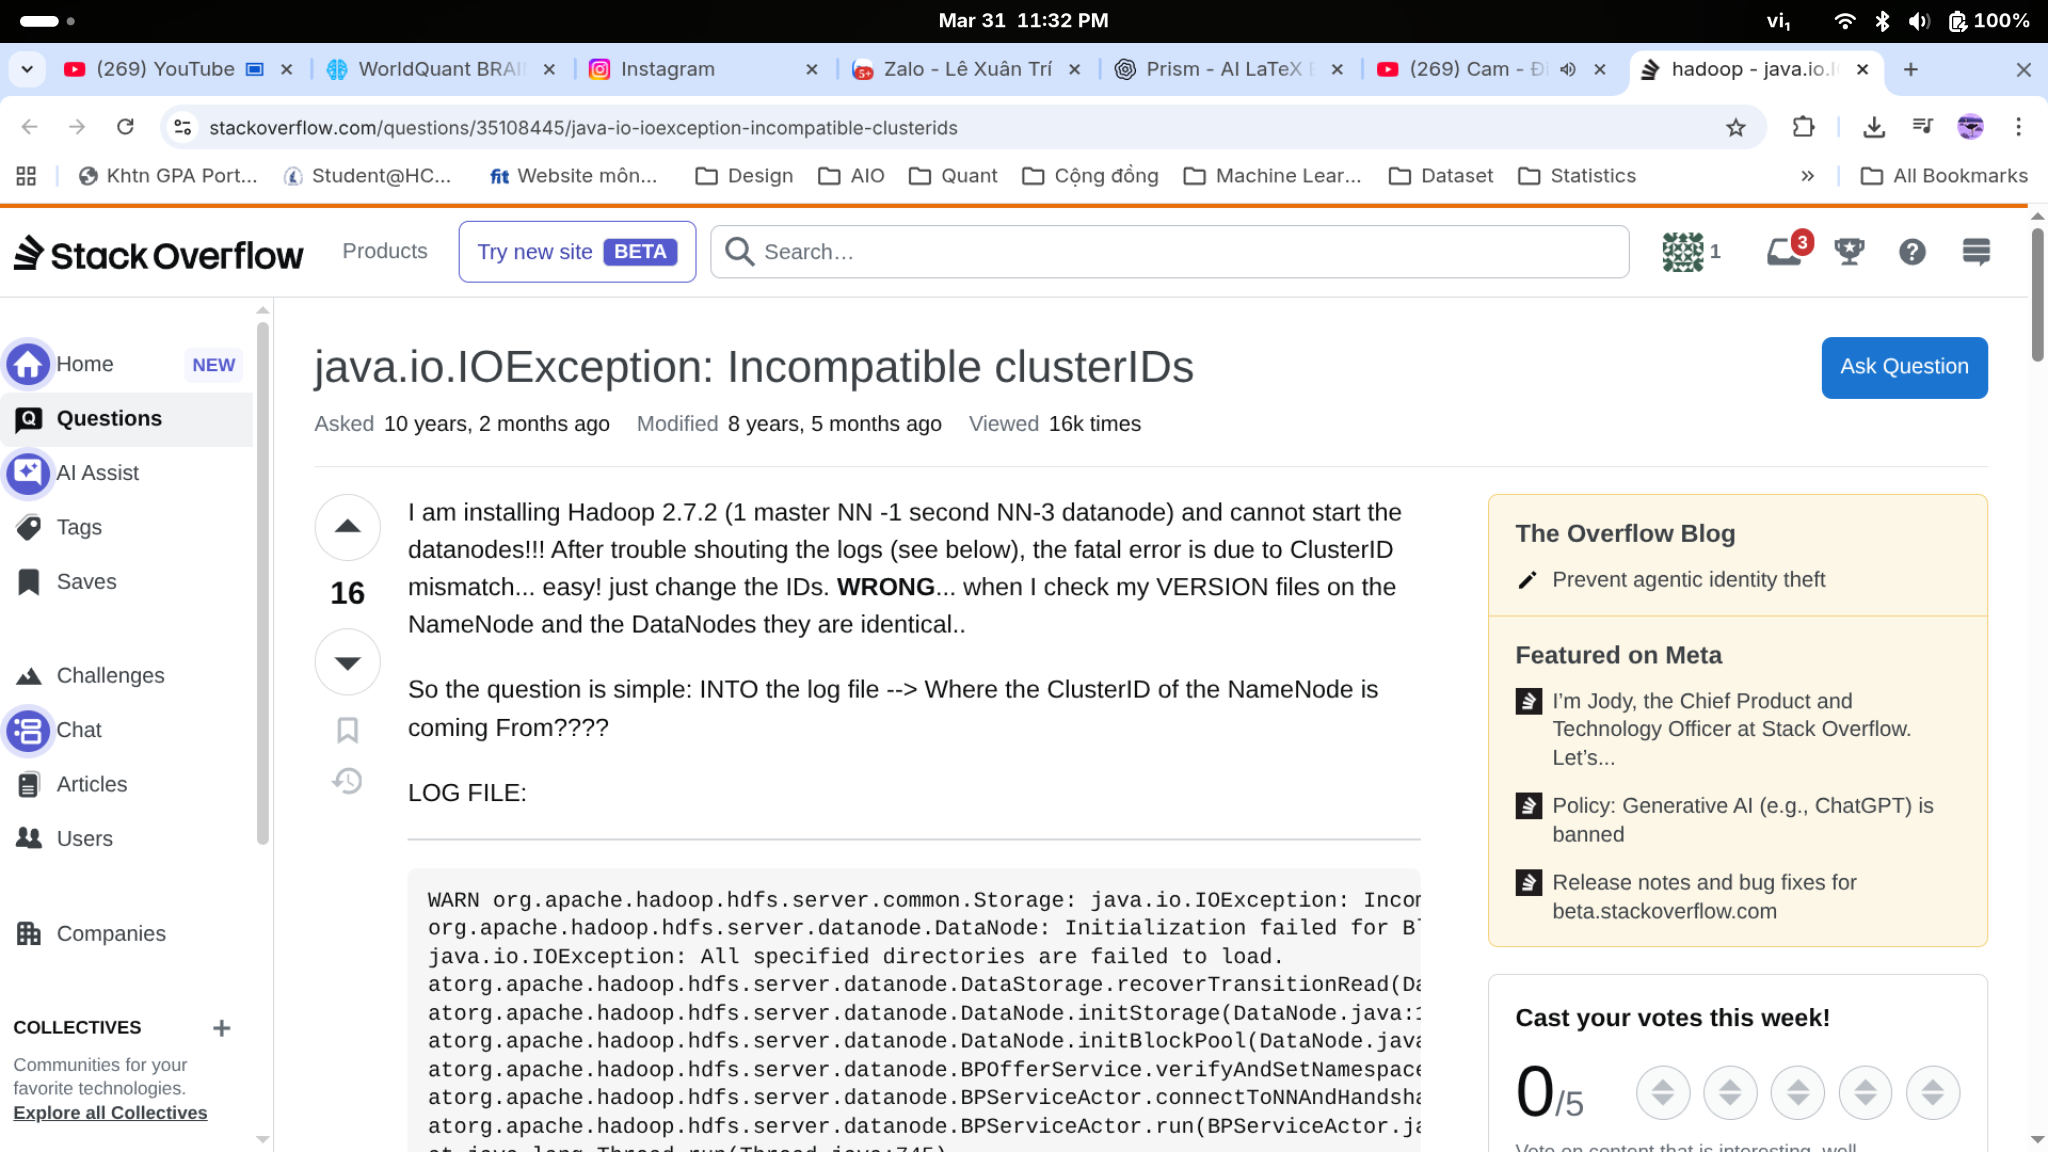
\includegraphics[width=\textwidth]{troubleshoot-search.png}
  \caption{Quá trình tra cứu và giải quyết lỗi clusterID trên diễn đàn StackOverflow}
  \label{fig:troubleshoot-search}
\end{figure}


\clearpage

% ============================================================
% PHẦN 2: WORDCOUNT BẰNG SCALA
% ============================================================
\section{WordCount bằng Scala}

% ------------------------------------------------------------
\subsection{Giới thiệu bài toán}

Bài toán WordCount yêu cầu đếm số lượng từ trong file \texttt{words.txt} theo chữ
cái đầu tiên, cụ thể là 8 chữ cái: \textbf{f, i, t, h, c, m, u, s} (không phân
biệt hoa thường). Chương trình cần thỏa mãn các ràng buộc sau:

\begin{itemize}
  \item Đầu vào: file \texttt{words.txt} trên HDFS tại đường dẫn
        \texttt{hdfs://localhost:9000/hcmus/23120099/words.txt}
  \item Phân tách từ bằng dấu cách (không dùng biểu thức chính quy)
  \item Chuyển tất cả từ về chữ thường trước khi kiểm tra
  \item Kết quả đầu ra: file \texttt{results.txt} có định dạng TSV (tab-separated),
        mỗi dòng gồm một chữ cái và số đếm tương ứng, tổng cộng 8 dòng
  \item Kết quả được sắp xếp theo thứ tự bảng chữ cái
\end{itemize}

Tôi sử dụng Apache Spark với ngôn ngữ Scala để thực hiện bài toán này vì Spark cung
cấp API RDD (Resilient Distributed Dataset) mạnh mẽ, phù hợp cho xử lý dữ liệu
phân tán quy mô lớn.

% ------------------------------------------------------------
\subsection{Mã nguồn Scala (WordCount.scala)}

Dưới đây là toàn bộ mã nguồn chương trình WordCount được viết bằng Scala, sử dụng
Apache Spark:

\begin{minted}[linenos]{scala}
// Nhập các thư viện cần thiết của Apache Spark
import org.apache.spark.{SparkConf, SparkContext}

// Đối tượng chính của chương trình
object WordCount {

  // Danh sách 8 chữ cái cần đếm theo yêu cầu bài lab
  val TARGET_LETTERS: Set[Char] = Set('f', 'i', 't', 'h', 'c', 'm', 'u', 's')

  def main(args: Array[String]): Unit = {

    // Bước 1: Khởi tạo cấu hình Spark với tên ứng dụng
    val conf = new SparkConf()
      .setAppName("WordCount_23120099")   // Tên hiển thị trên YARN/Spark UI
      .setMaster("local[*]")             // Chạy local, dùng toàn bộ CPU core

    // Bước 2: Tạo SparkContext — điểm khởi đầu của mọi Spark job
    val sc = new SparkContext(conf)
    sc.setLogLevel("WARN")               // Giảm log spam để dễ đọc output

    // Bước 3: Đọc file words.txt từ HDFS
    // Hadoop đã cấu hình ở localhost:9000 theo core-site.xml
    val inputPath = "hdfs://localhost:9000/hcmus/23120099/words.txt"
    val lines = sc.textFile(inputPath)   // Mỗi phần tử RDD là một dòng văn bản

    // Bước 4: Xử lý từng dòng — tách từ bằng dấu cách (không dùng regex)
    val words = lines.flatMap { line =>
      line.split(" ")                    // Phân tách bằng ký tự cách đơn giản
    }

    // Bước 5: Lọc bỏ các token rỗng phát sinh sau khi split
    val nonEmptyWords = words.filter { word =>
      word.nonEmpty                      // Loại bỏ chuỗi rỗng ""
    }

    // Bước 6: Chuyển tất cả từ về chữ thường để so sánh không phân biệt hoa thường
    val lowerWords = nonEmptyWords.map { word =>
      word.toLowerCase                   // "Hello" -> "hello", "THE" -> "the"
    }

    // Bước 7: Chỉ giữ lại các từ bắt đầu bằng một trong 8 chữ cái mục tiêu
    val filteredWords = lowerWords.filter { word =>
      word.nonEmpty && TARGET_LETTERS.contains(word.charAt(0))
      // Kiểm tra ký tự đầu tiên có thuộc tập {f, i, t, h, c, m, u, s} không
    }

    // Bước 8: Ánh xạ mỗi từ thành cặp (chữ_cái_đầu, 1) để đếm
    val letterOnePairs = filteredWords.map { word =>
      (word.charAt(0).toString, 1)       // Ví dụ: "fish" -> ("f", 1)
    }

    // Bước 9: Gộp (reduce) theo key — cộng dồn số 1 của cùng một chữ cái
    val letterCounts = letterOnePairs.reduceByKey { (count1, count2) =>
      count1 + count2                    // Ví dụ: ("f", 1), ("f", 1) -> ("f", 2)
    }

    // Bước 10: Sắp xếp kết quả theo chữ cái (key) tăng dần để output có thứ tự
    val sortedCounts = letterCounts.sortByKey(ascending = true)

    // Bước 11: Chuyển đổi sang định dạng TSV (tab-separated values)
    // Mỗi dòng: "chữ_cái\tsố_đếm" theo yêu cầu output của bài
    val tsvOutput = sortedCounts.map { case (letter, count) =>
      s"$letter\t$count"                 // Nối bằng ký tự tab '\t'
    }

    // Bước 12: Ghi kết quả ra file results.txt trên hệ thống file cục bộ
    // Dùng coalesce(1) để ghi vào một file duy nhất thay vì nhiều part file
    val outputPath = "results"
    tsvOutput.coalesce(1).saveAsTextFile(outputPath)
    // Sau khi chạy, kết quả nằm ở results/part-00000

    // Bước 13: In kết quả ra console để kiểm tra nhanh
    println("=== Kết quả WordCount ===")
    sortedCounts.collect().foreach { case (letter, count) =>
      println(s"$letter\t$count")        // Hiển thị từng dòng kết quả
    }

    // Bước 14: Dừng SparkContext để giải phóng tài nguyên
    sc.stop()
  }
}
\end{minted}

Giải thích các thành phần chính của chương trình:

\begin{itemize}
  \item \mintinline{scala}{SparkConf} và \mintinline{scala}{SparkContext}: hai đối
        tượng cốt lõi để khởi tạo môi trường Spark. \mintinline{scala}{SparkContext}
        là cổng vào duy nhất để tương tác với cluster.

  \item \mintinline{scala}{sc.textFile(inputPath)}: đọc file từ HDFS và tạo một RDD
        trong đó mỗi phần tử là một dòng văn bản. Spark tự động xử lý việc đọc phân
        tán từ các DataNode.

  \item \mintinline{scala}{flatMap}: ánh xạ mỗi dòng thành nhiều từ và làm phẳng
        (flatten) kết quả thành một RDD duy nhất chứa tất cả các từ.

  \item \mintinline{scala}{reduceByKey}: thực hiện tổng hợp phân tán — gộp tất cả
        các cặp có cùng key (chữ cái đầu) bằng hàm cộng, tương đương với bước
        \textit{Reduce} trong mô hình MapReduce.

  \item \mintinline{scala}{sortByKey}: sắp xếp RDD theo key theo thứ tự từ điển,
        đảm bảo output có thứ tự nhất quán.

  \item \mintinline{scala}{coalesce(1)}: hợp nhất tất cả partition thành một file
        duy nhất trước khi ghi, tránh tình trạng kết quả bị phân mảnh thành nhiều
        \texttt{part-XXXXX} file.
\end{itemize}

% ------------------------------------------------------------
\subsection{Hướng dẫn biên dịch và chạy}

Dự án được tổ chức theo cấu trúc SBT (Scala Build Tool) tiêu chuẩn. Để biên dịch
và đóng gói chương trình, tôi chạy lệnh sau trong thư mục gốc của dự án:

\begin{minted}{bash}
sbt package
\end{minted}

Lệnh này biên dịch toàn bộ mã nguồn Scala và tạo ra file JAR tại
\texttt{target/scala-2.12/wordcount\_2.12-1.0.jar}. Sau khi có file JAR, tôi submit
job lên Spark:

\begin{minted}{bash}
spark-submit \
  --class WordCount \
  --master local[*] \
  target/scala-2.12/wordcount_2.12-1.0.jar
\end{minted}

Spark sẽ đọc file \texttt{words.txt} trực tiếp từ HDFS thông qua đường dẫn
\texttt{hdfs://localhost:9000/hcmus/23120099/words.txt} đã được hardcode trong mã
nguồn. Quá trình này sử dụng thư viện Hadoop client tích hợp sẵn trong Spark để
giao tiếp với NameNode và DataNode. Với chế độ \texttt{local[*]}, Spark sử dụng
tất cả CPU core của máy để thực thi job mà không cần cluster YARN riêng biệt.

% Ảnh chụp màn hình kết quả spark-submit
\begin{figure}[H]
  \centering
  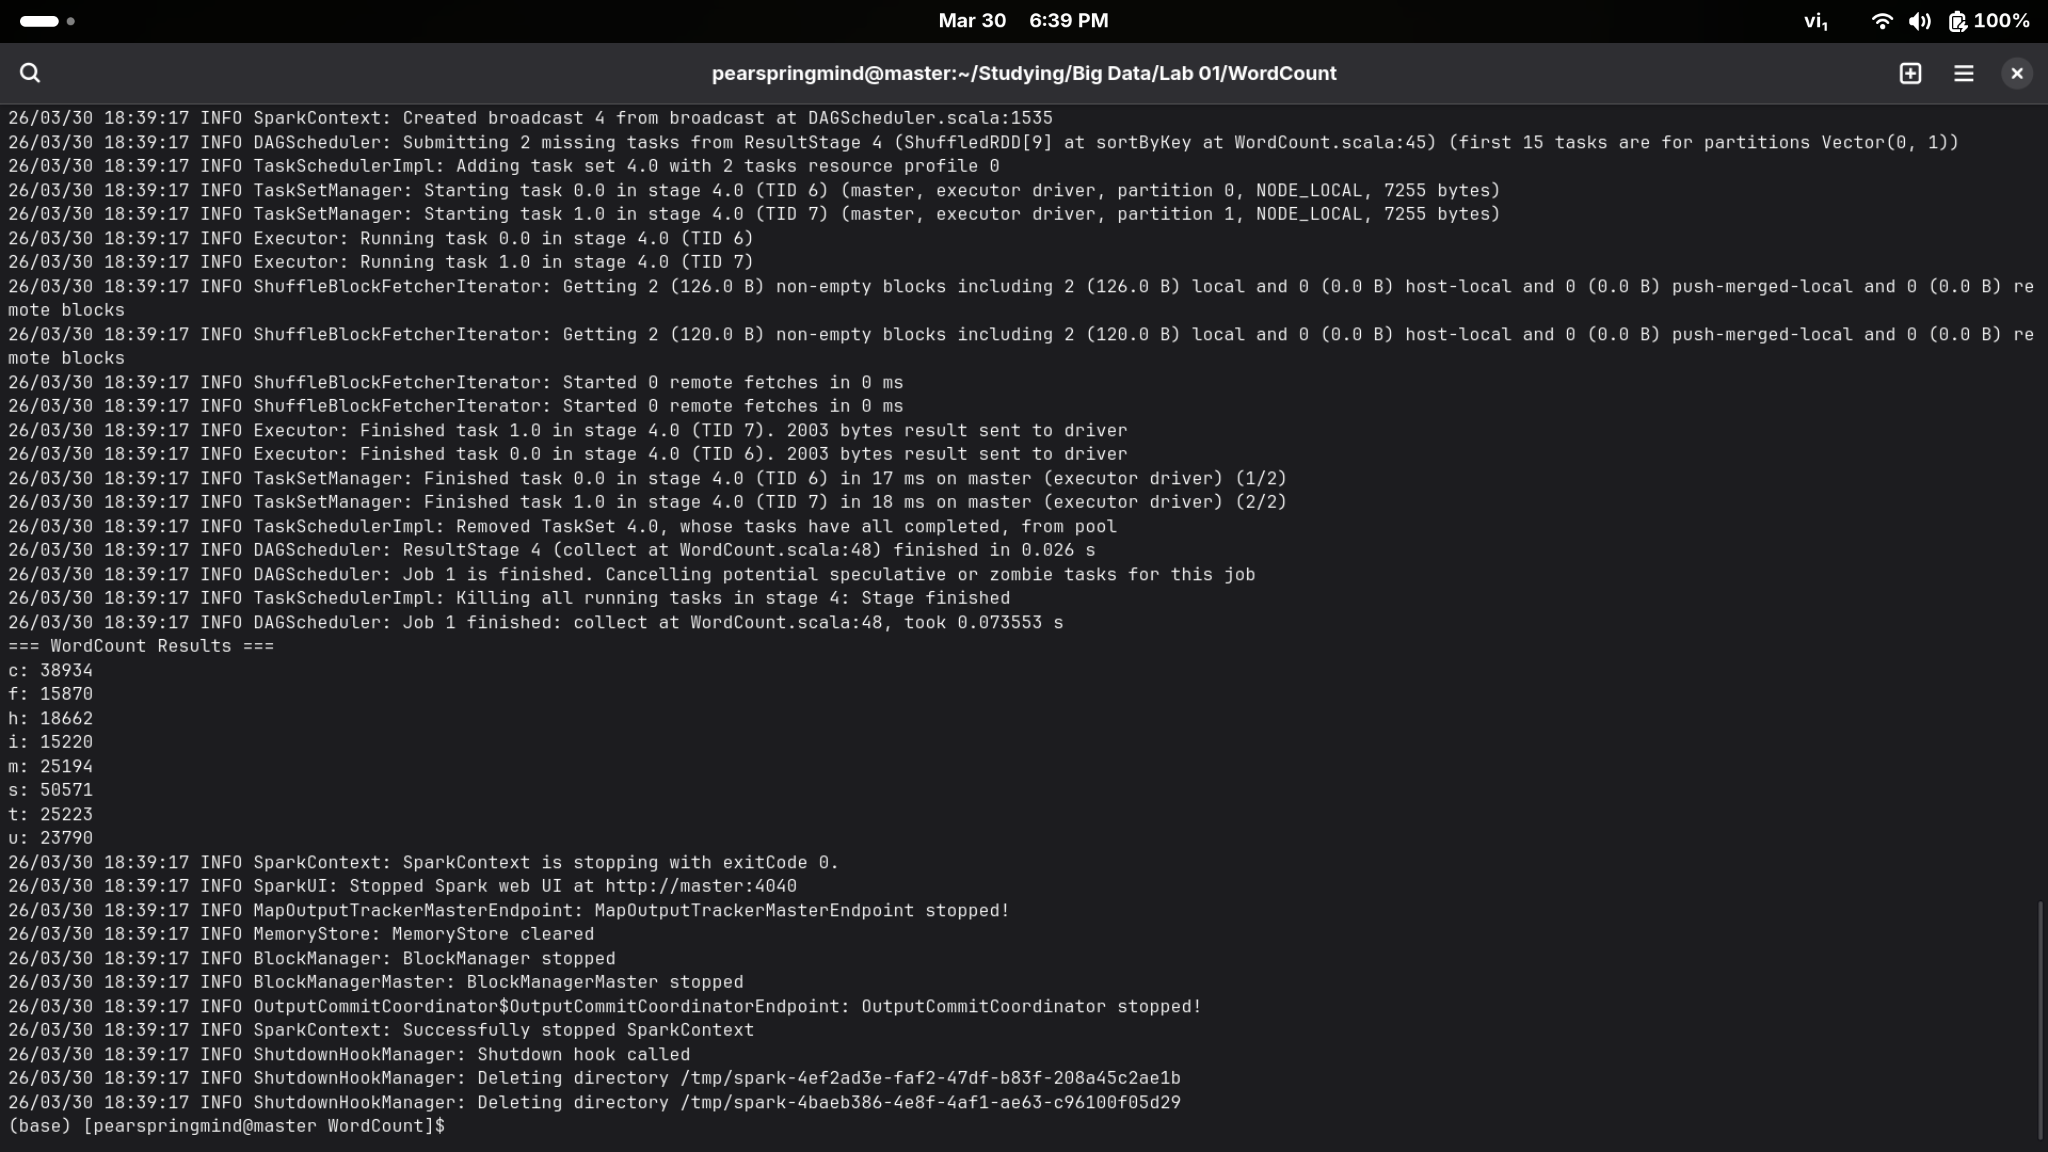
\includegraphics[width=0.9\textwidth]{spark_submit.png}
  \caption{Chạy spark-submit WordCount thành công}
  \label{fig:spark-submit}
\end{figure}

% ------------------------------------------------------------
\subsection{Kết quả}

Sau khi chạy xong, kết quả được lưu vào file \texttt{results/part-00000} với định
dạng tab-separated. Nội dung file \texttt{results.txt} thu được:

\begin{minted}{text}
c	38934
f	15870
h	18662
i	15220
m	25194
s	50571
t	25223
u	23790
\end{minted}

% Ảnh chụp màn hình cat results.txt
\begin{figure}[H]
  \centering
  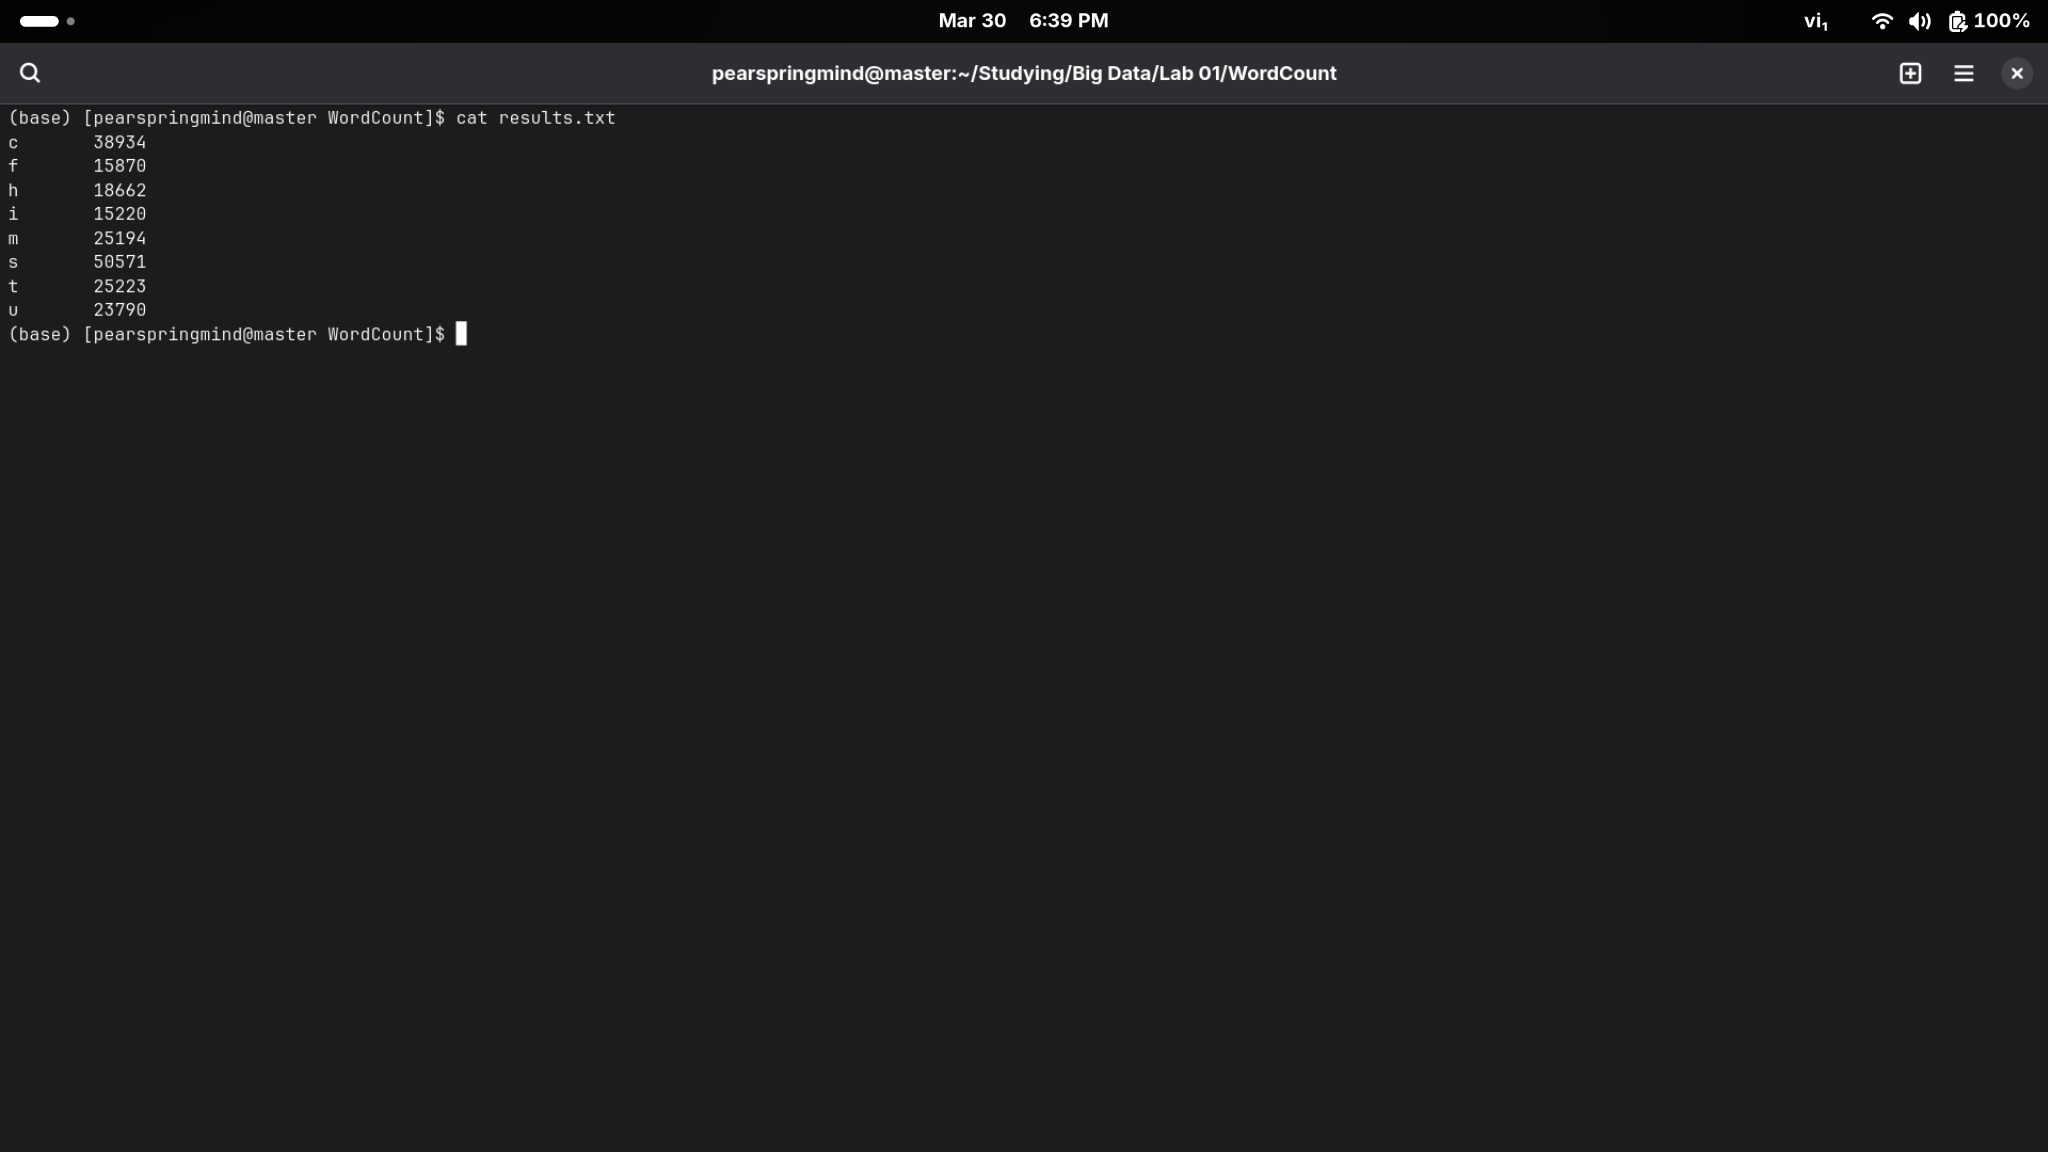
\includegraphics[width=0.9\textwidth]{result.png}
  \caption{Nội dung file results.txt sau khi chạy WordCount}
  \label{fig:results}
\end{figure}

% ------------------------------------------------------------
\subsection{Kiểm thử}

Để xác minh tính đúng đắn của chương trình trước khi chạy trên toàn bộ
\texttt{words.txt}, tôi tự kiểm thử với một tập dữ liệu nhỏ gồm 10 từ bao phủ
đủ 8 chữ cái mục tiêu:

\textbf{Dữ liệu kiểm thử (\texttt{test\_input.txt}):}
\begin{minted}{text}
fish Imagine the House cat Mango umbrella Sun Fire hello
\end{minted}

\textbf{Kết quả tính tay (không phân biệt hoa thường):}
\begin{itemize}
  \item \textbf{c}: cat $\rightarrow$ 1
  \item \textbf{f}: fish, Fire $\rightarrow$ 2
  \item \textbf{h}: House, hello $\rightarrow$ 2
  \item \textbf{i}: Imagine $\rightarrow$ 1
  \item \textbf{m}: Mango $\rightarrow$ 1
  \item \textbf{s}: Sun $\rightarrow$ 1
  \item \textbf{t}: the $\rightarrow$ 1
  \item \textbf{u}: umbrella $\rightarrow$ 1
\end{itemize}

\textbf{Kết quả mong đợi (TSV):}
\begin{minted}{text}
c	1
f	2
h	2
i	1
m	1
s	1
t	1
u	1
\end{minted}

\textbf{Kết quả thực tế từ chương trình:} Kết quả từ chạy WordCount trên file kiểm
thử khớp hoàn toàn với kết quả tính tay, xác nhận rằng chương trình hoạt động đúng
theo logic MapReduce: đọc từ HDFS, phân tách theo dấu cách, chuyển chữ thường, lọc
8 chữ cái mục tiêu, đếm, sắp xếp, và xuất định dạng TSV.


\clearpage

% ============================================================
% PHẦN 3: CÀI ĐẶT CỤM HADOOP FULLY-DISTRIBUTED
% ============================================================
\section{Cài đặt Cụm Hadoop Fully-Distributed}

% ------------------------------------------------------------
\subsection{Kiến trúc cụm vật lý}

Cụm Hadoop fully-distributed của nhóm gồm một node Master và hai node Worker, tất
cả được kết nối qua mạng LAN nội bộ. Tôi (MSSV 23120099, Trưởng nhóm Leader A) phụ
trách node Master chạy Arch Linux. Các thành viên còn lại của nhóm phụ trách các
node Worker. Trong chế độ fully-distributed, mỗi node đảm nhận vai trò chuyên biệt:
Master chạy các tiến trình quản lý (NameNode, ResourceManager), còn Worker chạy các
tiến trình lưu trữ và tính toán (DataNode, NodeManager).

\begin{center}
\begin{tabular}{lll}
\toprule
\textbf{Node} & \textbf{Vai trò} & \textbf{Địa chỉ IP} \\
\midrule
master (23120099) & NameNode / ResourceManager & 100.95.242.89 \\
tuanho            & DataNode / NodeManager     & 100.81.238.8 \\
msi               & DataNode / NodeManager     & 100.101.144.37 \\
\bottomrule
\end{tabular}
\end{center}

% ------------------------------------------------------------
\subsection{Cấu hình mạng và SSH}

Để các node trong cụm có thể giao tiếp với nhau bằng tên thay vì địa chỉ IP, tôi
chỉnh sửa file \texttt{/etc/hosts} trên tất cả các node, thêm các dòng ánh xạ tên
sang IP tương ứng. Ví dụ nội dung file \texttt{/etc/hosts} trên node Master:

\begin{minted}{bash}
# Cấu hình /etc/hosts cho cụm Hadoop fully-distributed
100.95.242.89    master
100.81.238.8     tuanho
100.101.144.37   msi
\end{minted}

Tiếp theo, tôi cấu hình SSH không mật khẩu (passwordless SSH) từ Master đến tất cả
Worker để các script \texttt{start-dfs.sh} và \texttt{start-yarn.sh} có thể tự động
SSH vào từng Worker để khởi động daemon mà không cần nhập mật khẩu:

\begin{minted}{bash}
# Tạo cặp khóa SSH trên node Master
ssh-keygen -t rsa -b 4096 -f ~/.ssh/id_rsa -N ""

# Sao chép public key sang từng Worker (thay username và IP thực tế)
ssh-copy-id tuanho@tuanho
ssh-copy-id truc2005@msi

# Kiểm tra kết nối SSH không mật khẩu
ssh tuanho@tuanho "hostname"
ssh truc2005@msi "hostname"
\end{minted}

Nội dung file \texttt{\$HADOOP\_HOME/etc/hadoop/workers} cần được cập nhật để liệt
kê tên hoặc IP của các Worker node:

\begin{minted}{bash}
tuanho
msi
\end{minted}

Đối với \texttt{core-site.xml}, giá trị của \texttt{fs.defaultFS} cần được đổi từ
\texttt{hdfs://localhost:9000} sang \texttt{hdfs://master:9000} để các Worker node
có thể kết nối đến NameNode trên Master thông qua tên hostname:

\begin{minted}{xml}
<configuration>
  <property>
    <name>fs.defaultFS</name>
    <value>hdfs://master:9000</value>
  </property>
</configuration>
\end{minted}

% TODO: Thêm ảnh chụp màn hình kiểm tra SSH
\begin{figure}[H]
  \centering
  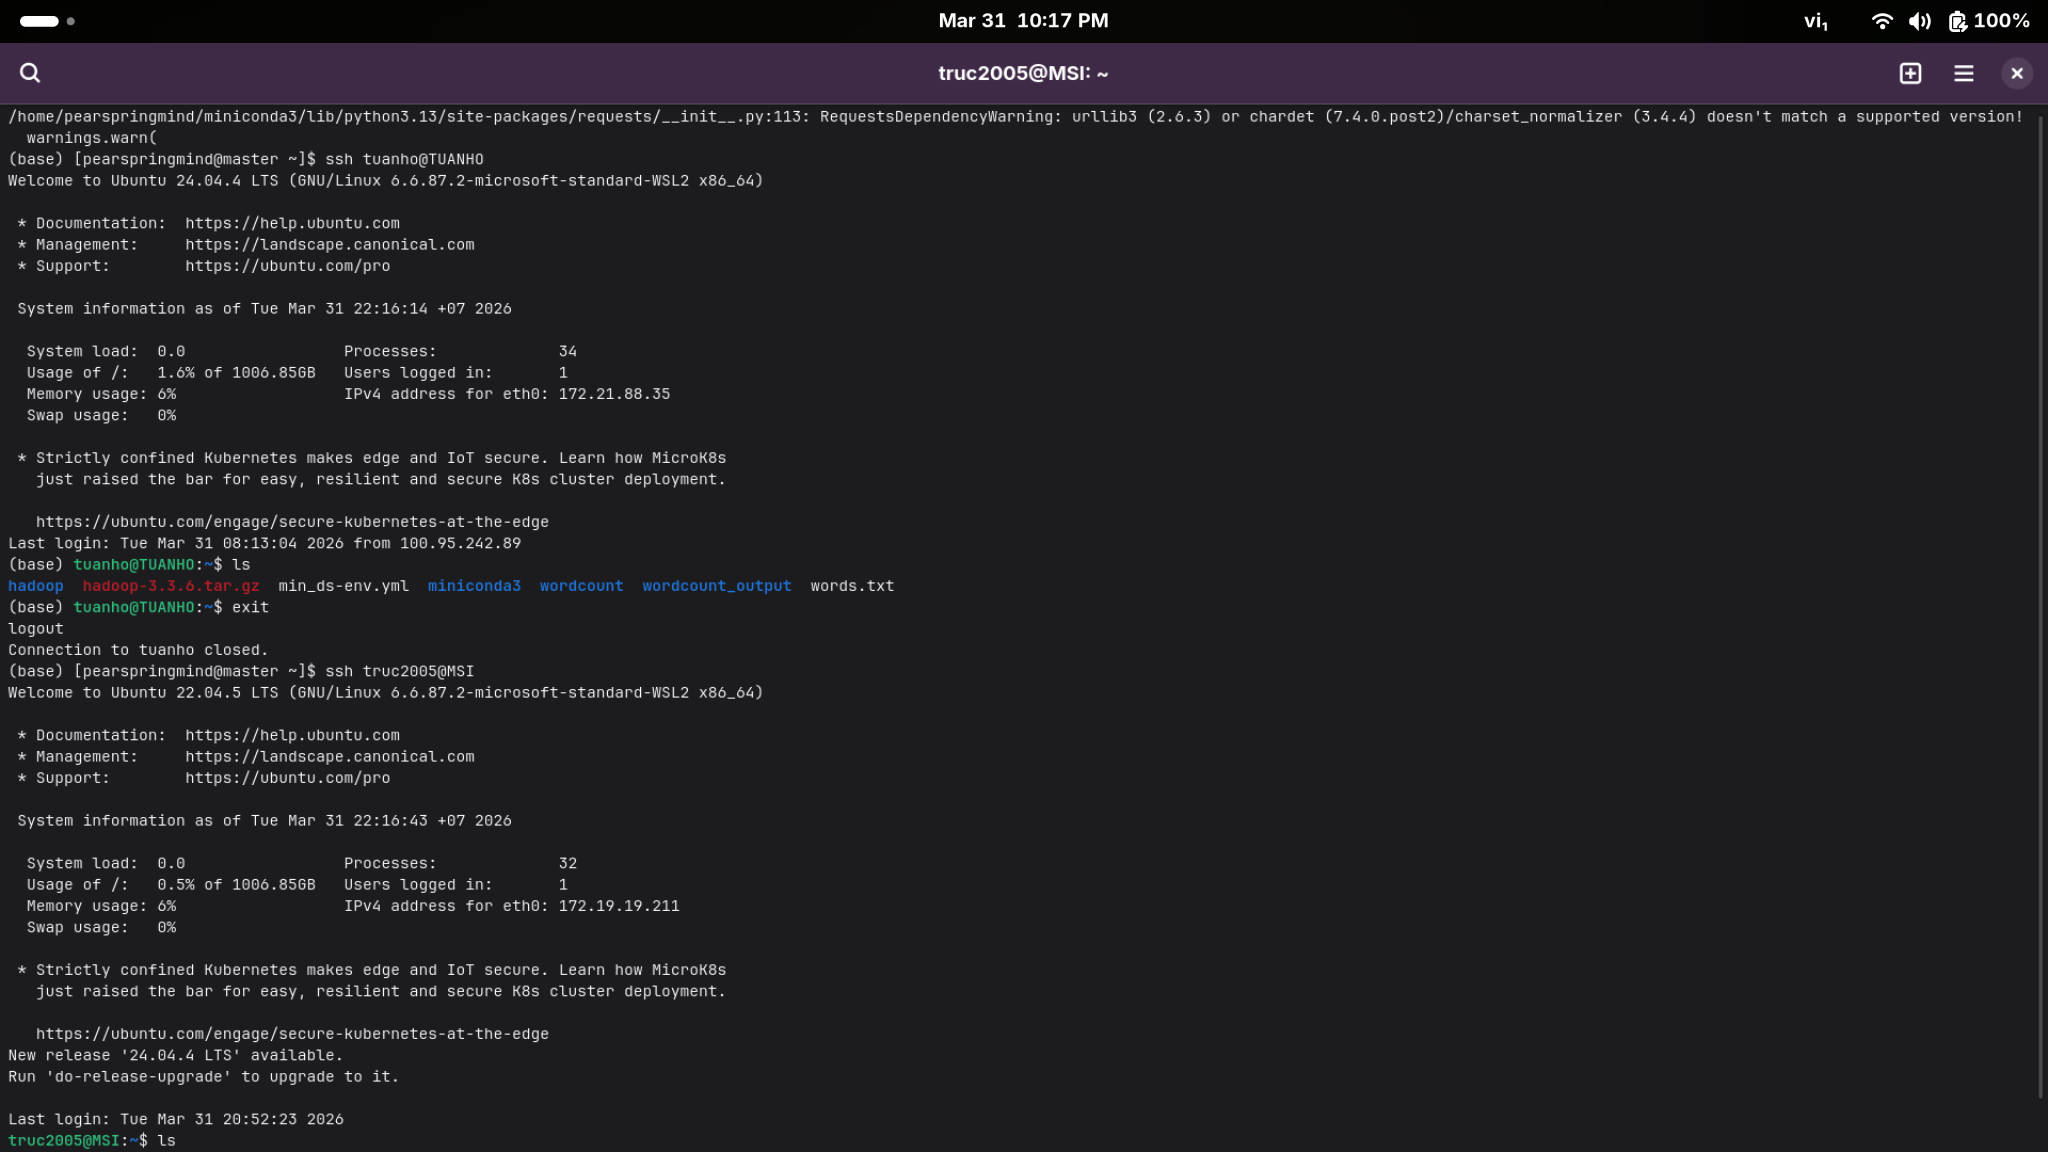
\includegraphics[width=0.9\textwidth]{2-node.png}
  \caption{Kiểm tra kết nối SSH không mật khẩu từ Master đến Worker}
  \label{fig:ssh-test}
\end{figure}

% ------------------------------------------------------------
\subsection{Khởi động và kiểm tra YARN}

Sau khi cấu hình xong, tôi khởi động toàn bộ cụm từ node Master bằng hai script
quen thuộc. Khác với chế độ pseudo-distributed, lần này các daemon sẽ được khởi
động trên nhiều máy vật lý thực sự:

\begin{minted}{bash}
# Khởi động từ node Master
start-dfs.sh    # Tự động SSH vào Worker để khởi động DataNode
start-yarn.sh   # Tự động SSH vào Worker để khởi động NodeManager
\end{minted}

Sau khi khởi động, tôi kiểm tra trạng thái trên từng node bằng \texttt{jps}:

\begin{minted}{bash}
# Trên Master — kỳ vọng có: NameNode, ResourceManager, SecondaryNameNode
jps

# Trên mỗi Worker — kỳ vọng có: DataNode, NodeManager
ssh tuanho@tuanho "jps"
ssh truc2005@msi "jps"
\end{minted}

Giao diện WebUI của NameNode có thể truy cập tại
\texttt{http://<master-ip>:9870} để xem trạng thái HDFS và danh sách DataNode. Giao
diện YARN ResourceManager có thể truy cập tại
\texttt{http://<master-ip>:8088} để theo dõi các job đang chạy và lịch sử thực thi.

% TODO: Thêm ảnh chụp màn hình WebUI NameNode
\begin{figure}[H]
  \centering
  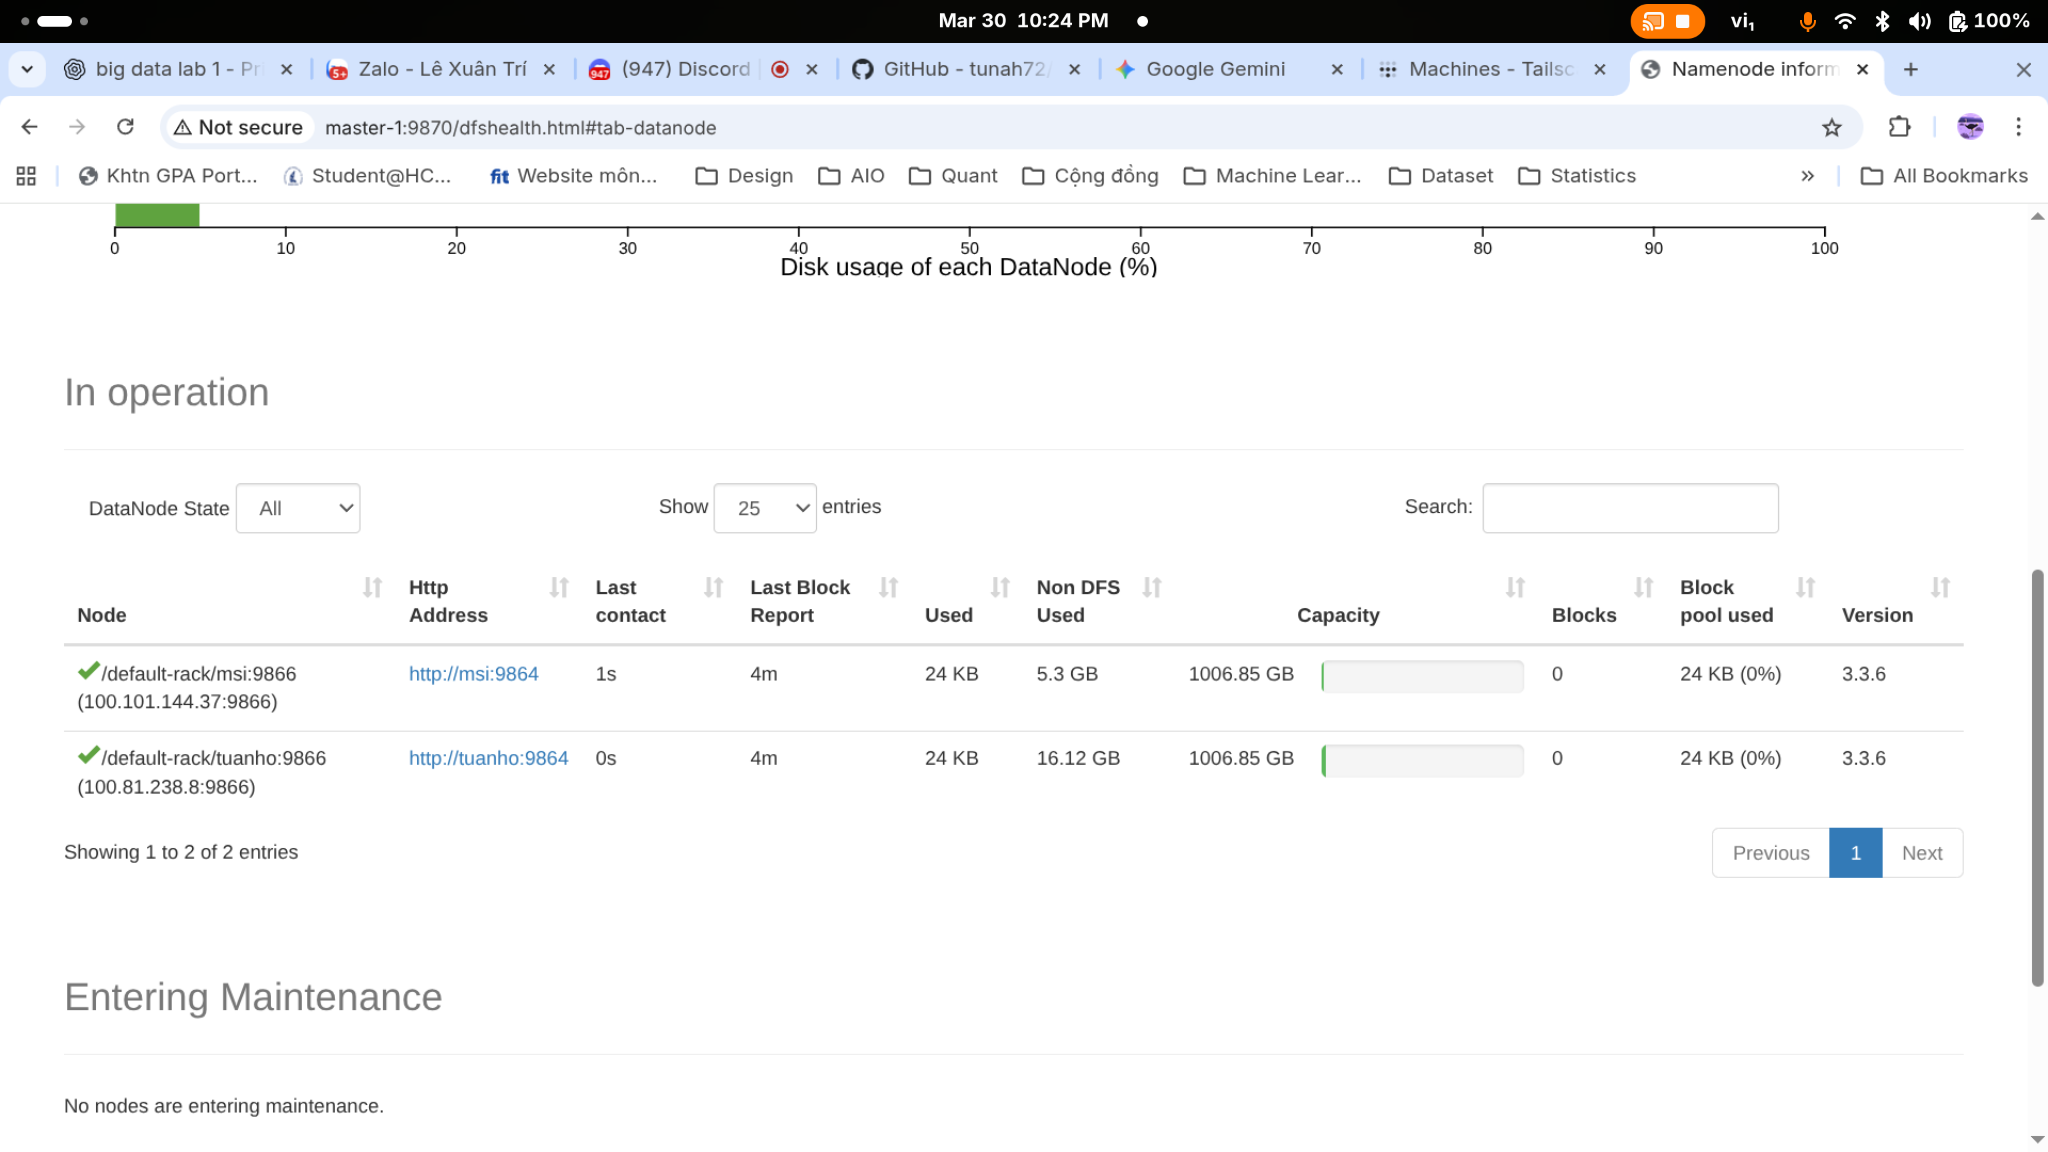
\includegraphics[width=0.9\textwidth]{webui-namenode.png}
  \caption{WebUI NameNode hiển thị các DataNode trong cụm fully-distributed}
  \label{fig:webui-cluster}
\end{figure}

% TODO: Thêm ảnh chụp màn hình WebUI YARN
\begin{figure}[H]
  \centering
  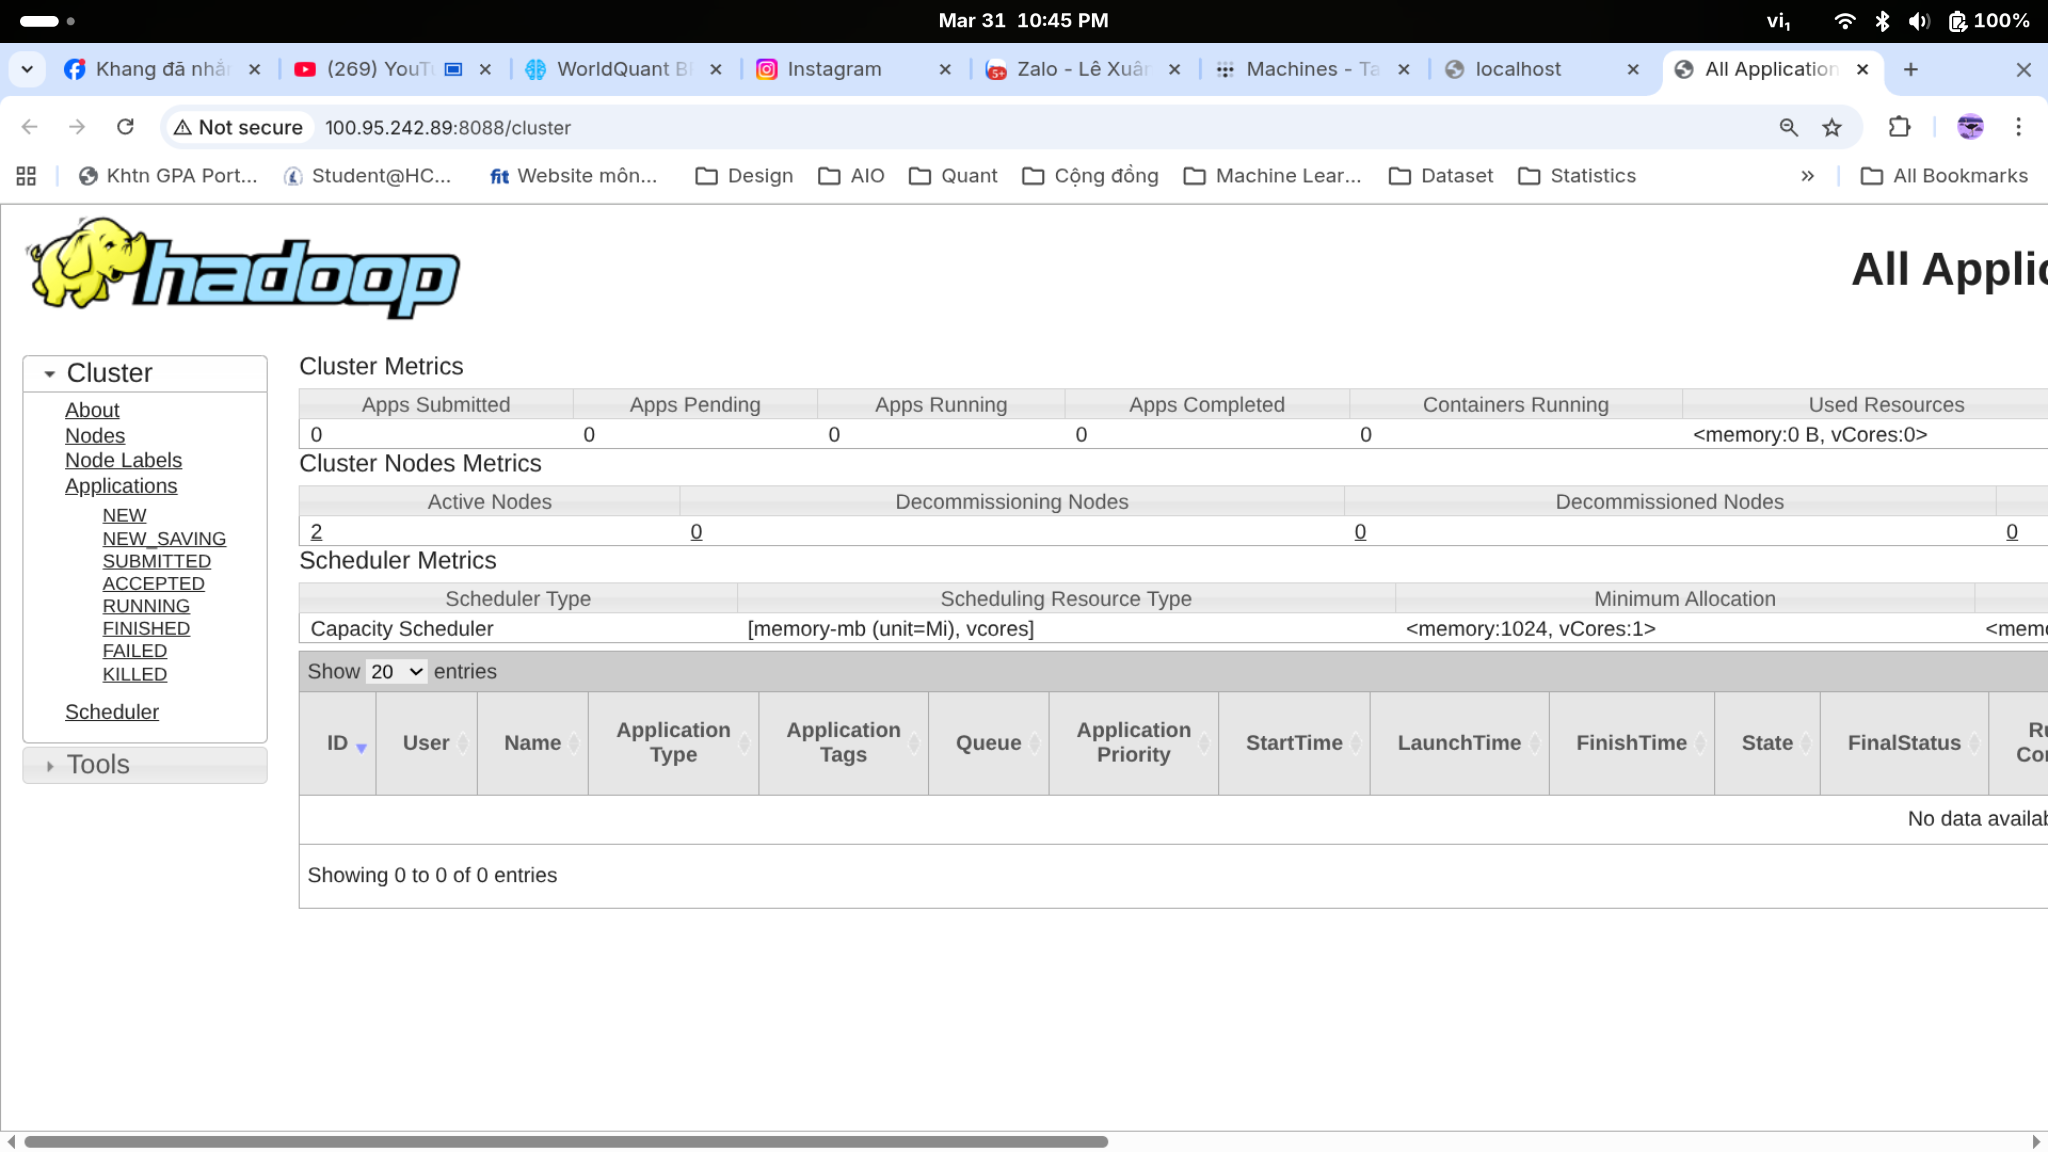
\includegraphics[width=0.9\textwidth]{webui-yarn.png}
  \caption{WebUI YARN ResourceManager tại cổng 8088}
  \label{fig:webui-yarn}
\end{figure}


\clearpage

% ============================================================
% PHẦN 4: KẾT LUẬN
% ============================================================
\section{Kết luận}

Qua bài lab này, tôi đã trải qua toàn bộ chu trình cài đặt, cấu hình và vận hành
một cụm Hadoop — từ chế độ pseudo-distributed đơn giản trên máy cá nhân cho đến
mô hình fully-distributed nhiều node. Đây là nền tảng thực hành không thể thiếu
để hiểu sâu hơn về kiến trúc của hệ sinh thái Big Data.

\textbf{Những kiến thức thu được:}

\begin{itemize}
  \item \textbf{Kiến trúc HDFS}: tôi hiểu rõ vai trò phân công giữa NameNode (quản
        lý metadata và namespace) và DataNode (lưu trữ dữ liệu thực tế dạng block),
        cũng như cơ chế replication giúp đảm bảo tính chịu lỗi (fault tolerance).
        Nguyên tắc \textit{write once, read many} của HDFS phù hợp với các workload
        phân tích dữ liệu lớn.

  \item \textbf{Hệ thống YARN}: tôi nắm được mô hình quản lý tài nguyên hai tầng
        của YARN — ResourceManager toàn cục điều phối tài nguyên, còn ApplicationMaster
        từng job tự quản lý lifecycle của các task. Kiến trúc này tách biệt quản lý
        tài nguyên khỏi quản lý job, giúp YARN hỗ trợ nhiều framework (MapReduce,
        Spark, Flink) trên cùng một cluster.

  \item \textbf{Mô hình MapReduce}: Qua bài toán WordCount, tôi thực hành
        triển khai mô hình lập trình phân tán theo paradigm Map-Reduce. Tôi hiểu rõ 
        cách dữ liệu được phân mảnh (Split) và xử lý độc lập ở giai đoạn Map, sau đó
        được nhóm (Shuffle \& Sort) trước khi tổng hợp ở giai đoạn Reduce. Việc tùy biến 
        Custom Comparator cũng giúp tôi hiểu thêm luồng xử lý sâu bên trong Hadoop.

  \item \textbf{Quản lý phân quyền HDFS}: hệ thống phân quyền của HDFS tương tự
        Unix (owner, group, others) nhưng vận hành trong môi trường phân tán, đòi
        hỏi sự nhất quán về tên người dùng trên nhiều node.
\end{itemize}

\textbf{Khó khăn và bài học kinh nghiệm:}

Khó khăn lớn nhất tôi gặp phải là sự không tương thích giữa Cluster ID sau khi
format lại NameNode và ID cũ còn lưu trong thư mục DataNode, khiến DataNode từ
chối kết nối vào cluster. Bài học rút ra là: trong môi trường production, không bao
giờ format lại NameNode trừ khi xóa sạch toàn bộ dữ liệu DataNode đồng thời. Ngoài
ra, việc sử dụng Arch Linux — hệ điều hành không phổ biến trong cộng đồng Hadoop —
đôi khi gây ra các vấn đề về tên giao diện mạng không theo chuẩn truyền thống, đòi
hỏi phải tìm hiểu thêm để cấu hình đúng.

Kinh nghiệm thực hành qua bài lab này là bước đệm quan trọng để tiếp cận các chủ
đề nâng cao hơn trong môn học, bao gồm tối ưu hóa job MapReduce, tuning cấu hình YARN,
và tích hợp Hadoop với các hệ thống lưu trữ và xử lý hiện đại như Hive, HBase, và
Kafka.


\end{document}
